% BU ECE template for MS thesis and PhD dissertation.
%
%==========================================================================%
% MAIN PREAMBLE 
%==========================================================================%
\documentclass[12pt,letterpaper]{report}          % Single-sided printing for the library
%\documentclass[12pt,twoside]{report} % Double-sided printing
\usepackage[intlimits]{amsmath}
\usepackage{amsthm}
\usepackage{amsfonts,amssymb}
\DeclareSymbolFontAlphabet{\mathbb}{AMSb}
%\usepackage{natbib}
\usepackage{apalike}
\usepackage{float}
\usepackage[bf]{caption}       
\setcaptionmargin{0.5in}
\usepackage{fancyhdr}
%\usepackage{fancyheadings}
\usepackage{fancybox}
\usepackage{ifthen}
\usepackage{bu_ece_thesis}
\usepackage{url}
\usepackage{lscape,afterpage}
\usepackage{xspace}
\usepackage{epstopdf} 
%\usepackage{subfig}
%==========================================================================%
%%% graphicx and pdf creation
\usepackage{graphicx}
\usepackage{appendix}
\usepackage{pdfpages}

\setcounter{tocdepth}{3}
\usepackage{subfigure}
\usepackage{xspace}
\usepackage{algorithm}
\usepackage{algpseudocode}
\usepackage[colorlinks=true,bookmarks=false]{hyperref}
%%%%%%%%%%%%%%%% macros %%%%%%%%%%%%%%%%%%%%%%%%%%

%%%%%%%%%%%%%%%%% Prelim %%%%%%%%%%%%%%%%%%%%%%%%%
\newcommand{\AP}{\ensuremath{AP}\xspace}
\newcommand{\lang}{\mathcal{L}}
\newcommand{\false}{\texttt{false}}
\newcommand{\true}{\texttt{true}}

\newcommand{\naturalnumber}{\mathbb{N}}
\newcommand{\integer}{\mathbb{Z}}
\newcommand{\rational}{\mathbb{Q}}
\newcommand{\reals}{\mathbb{R}}
\newcommand{\Bool}{\mathbb{B}}

\newcommand{\globally}{{\textbf{G}}\xspace} 
\newcommand{\eventually}{{\textbf{F}}\xspace}
\newcommand{\allpaths}{{\textbf{A}}\xspace}
\newcommand{\existpath}{{\textbf{E}}\xspace}
\newcommand{\until}{{\textbf{U}}\xspace}
\newcommand{\nextstate}{{\textbf{X}}\xspace}

%\newtheorem{proposition}{Proposition}[section]
%\newtheorem{theorem}{Theorem}[section] % use section or use nothing?
%\newtheorem{lemma}{Lemma}[section] 
%\newtheorem{mydef}{Definition}[section]
%\newtheorem{rmark}{Remark}[section]
%\renewenvironment{remark}{\begin{rmark}\rm}{\qed\end{rmark}}

%\newcommand{\qed}{\mbox{} $\Box$}
%\newenvironment{proof}{{\it Proof:}}{\qed}
%\newtheorem{proposition}[theorem]{Proposition}
%\newtheorem{xmpl}{Example}
%\newenvironment{example}{\begin{xmpl}}{\end{xmpl}}

%%%%%%%%%%%%%%%%%%%%%%%%%%%%%%%%%%%%%%%%%%

\renewcommand{\algorithmicrequire}{\textbf{Input:}}
\renewcommand{\algorithmicensure}{\textbf{Output:}}

%\newcommand{\keywords}[1]{\par\addvspace\baselineskip
%\noindent\keywordname\enspace\ignorespaces#1}

\newcommand{\comment}[1]{}

%%%%%%%%%%%%%%%%%%%%% MISC %%%%%%%%%%%%%%%%%%%%%%%%%%%%%%%%%%%%%%%%


  
\newcommand{\keywords}[1]{\par\addvspace\baselineskip
\noindent\keywordname\enspace\ignorespaces#1}

\theoremstyle{definition}
\newtheorem{definition}{Definition}[section]

\newtheorem{theorem}{Theorem}[section]
\newtheorem{corollary}{Corollary}[theorem]
\newtheorem{lemma}[theorem]{Lemma}
 
\theoremstyle{remark}
\newtheorem*{remark}{Remark}

%\usepackage{psfrag}
%\DeclareGraphicsExtensions{.eps}   % extension for included graphics
%\usepackage{thumbpdf}              % thumbnails for ps2pdf
%\usepackage[ps2pdf,                % hyper-references for ps2pdf
%bookmarks=true,%                   % generate bookmarks ...
%bookmarksnumbered=true,%           % ... with numbers
%hypertexnames=false,%              % needed for correct links to figures !!!
%breaklinks=true,%                  % breaks lines, but links are very small
%linkbordercolor={0 0 1},%          % blue frames around links
%pdfborder={0 0 112.0}]{hyperref}%  % border-width of frames 
%                                   % will be multiplied with 0.009 by ps2pdf
%\hypersetup{
%  pdfauthor   = {Joe Graduate <joe.graduate@bu.edu>},
%  pdftitle    = {dissertation.pdf},
%  pdfsubject  = {doctoral dissertations},
%  pdfkeywords = {mathematics, science, technology},
%  pdfcreator  = {LaTeX with hyperref package},
%  pdfproducer = {dvips + ps2pdf}
%}
%==========================================================================%
% customized commands can be placed here
%\newcommand{\figref}[1]{Figure~\ref{#1}}
%\newcommand{\chapref}[1]{Chapter~\ref{#1}}
%\newcommand{\latex}{\LaTeX\xspace}
%==========================================================================%

%==========================================================================%
% BEGIN
%==========================================================================%
\begin{document}

% The preliminary pages
% This file contains all the necessary setup and commands to create
% the preliminary pages according to the buthesis.sty option.

\title{Safety-Aware Apprenticeship Learning}

\author{Weichao Zhou}

% Type of document prepared for this degree:
%   1 = Master of Science thesis,
%   2 = Doctor of Philisophy dissertation.
%   3 = Master of Science thesis and Doctor of Philisophy dissertation.
\degree=1

\prevdegrees{B.S., Fudan University, 2012}

\department{Department of Electrical and Computer Engineering}

% Degree year is the year the diploma is expected, and defense year is
% the year the dissertation is written up and defended. Often, these
% will be the same, except for January graduation, when your defense
% will be in the fall of year X, and your graduation will be in
% January of year X+1
\defenseyear{2018}
\degreeyear{2018}

% For each reader, specify appropriate label {First, Second, Third},
% then name, and title. IMPORTANT: The title should be:
%   "Professor of Electrical and Computer Engineering",
% or similar, but it MUST NOT be:
%   Professor, Department of Electrical and Computer Engineering"
% or you will be asked to reprint and get new signatures.
% Warning: If you have more than five readers you are out of luck,
% because it will overflow to a new page. You may try to put part of
% the title in with the name.
\reader{First}{Wenchao Li}{Assistant Professor of Electrical and Computer Engineering\\Assistant Professor of Systems Engineering
}
\reader{Second}{Brian Kulis}{Assistant Professor of Electrical and Computer Engineerings\\Assistant Professor of Systems Engineering\\Assistant Professor of Computer Science
}
\reader{Third}{Yannis Paschalidis}{Professor of Electrical and Computer Engineering\\Professor of Systems Engineering\\Professor of Biomedical Engineering
}

% The Major Professor is the same as the first reader, but must be
% specified again for the abstract page. Up to 4 Major Professors
% (advisors) can be defined. 
\numadvisors=1
\majorprof{Wenchao Li}{{Assistant Professor of Electrical and Computer Engineering}}
%\majorprofb{First M. Last, PhD}{{Professor of Computer Science}}
%\majorprofc{First M. Last, PhD}{{Professor of Astronomy}}
%\majorprofd{First M. Last, PhD}{{Professor of Biomedical Engineering}}

%%%%%%%%%%%%%%%%%%%%%%%%%%%%%%%%%%%%%%%%%%%%%%%%%%%%%%%%%%%%%%%%  

%                       PRELIMINARY PAGES
% According to the BU guide the preliminary pages consist of:
% title, copyright (optional), approval,  acknowledgments (opt.),
% abstract, preface (opt.), Table of contents, List of tables (if
% any), List of illustrations (if any). The \tableofcontents,
% \listoffigures, and \listoftables commands can be used in the
% appropriate places. For other things like preface, do it manually
% with something like \newpage\section*{Preface}.

% This is an additional page to print a boxed-in title, author name and
% degree statement so that they are visible through the opening in BU
% covers used for reports. This makes a nicely bound copy. Uncomment only
% if you are printing a hardcopy for such covers. Leave commented out
% when producing PDF for library submission.
%\buecethesistitleboxpage

% Make the titlepage based on the above information.  If you need
% something special and can't use the standard form, you can specify
% the exact text of the titlepage yourself.  Put it in a titlepage
% environment and leave blank lines where you want vertical space.
% The spaces will be adjusted to fill the entire page.
\maketitle
\cleardoublepage

% The copyright page is blank except for the notice at the bottom. You
% must provide your name in capitals.
\copyrightpage
\cleardoublepage

% Now include the approval page based on the readers information
\approvalpage
\cleardoublepage

% Here goes your favorite quote. This page is optional.
%\newpage
%\thispagestyle{empty}
%\phantom{.}
\vspace{4in}

\begin{singlespace}
\begin{quote}
  \textit{Facilis descensus Averni;}\\
  \textit{Noctes atque dies patet atri janua Ditis;}\\*
  \textit{Sed revocare gradum, superasque evadere ad auras,}\\
  \textit{Hoc opus, hic labor est.}\hfill{Virgil (from Don's thesis!)}
\end{quote}
\end{singlespace}

% \vspace{0.7in}
%
% \noindent
% [The descent to Avernus is easy; the gate of Pluto stands open night
% and day; but to retrace one's steps and return to the upper air, that
% is the toil, that the difficulty.]

%\cleardoublepage

% The acknowledgment page should go here. Use something like
% \newpage\section*{Acknowledgments} followed by your text.
\newpage
%%%%%%%%%
%Acknowledge starts from page 4. Page 3 is for the approval page
%%%%%%%%%
\section*{\centerline{Acknowledgments}}
I want to express my deepest appreciation to my advisor, Professor Wenchao Li.
During my two-year master's studies, he has always been a great mentor for me. 
He set an example of excellence as a researcher, instructor and role model.
My experiences in his group have always been rewarding. 
Conducting researches under his guidance motivates me to refine my skills and set a high standard for myself. 
I cherish this opportunity for professional and personal development that he has provided me.

I would like to thank my thesis committee members for providing me support through this process. 
Your suggestions and feedback have been invaluable for me.

I also want to thank our department for providing me with such an open and resourceful environment. 
I'm so glad that I will be able to continue enjoying my time here as a PhD student.

Last but not least, I can not tell how grateful I am to my parents.
I would not have been here without your encouragement. You believe in me and always want the best for me.
You are oceans away, yet your love is close.

\vskip 1in

\cleardoublepage

% The abstractpage environment sets up everything on the page except
% the text itself.  The title and other header material are put at the
% top of the page, and the supervisors are listed at the bottom.  A
% new page is begun both before and after.  Of course, an abstract may
% be more than one page itself.  If you need more control over the
% format of the page, you can use the abstract environment, which puts
% the word "Abstract" at the beginning and single spaces its text.

\begin{abstractpage}
% ABSTRACT
It is well acknowledged in the AI community that finding a good reward function for reinforcement learning is extremely challenging. Apprenticeship learning (AL) is a class of ``learning from demonstration'' techniques where the reward function of a Markov Decision Process (MDP) is unknown to the learning agent and the agent uses inverse reinforcement learning (IRL) methods to recover expert policy from a set of expert demonstrations. However, as the agent learns exclusively from observations, given a constraint on the probability of the agent running into unwanted situations, there is no verification, nor guarantee, for the learnt policy on the satisfaction of the restriction. In this dissertation, we study the problem of how to guide AL to learn a policy that is inherently safe while still meeting its learning objective. By combining formal methods with imitation learning, a Counterexample-Guided Apprenticeship Learning algorithm is proposed. We consider a setting where the unknown reward function is assumed to be a linear combination of a set of state features, and the safety property is specified in Probabilistic Computation Tree Logic (PCTL). By embedding probabilistic model checking inside AL, we propose a novel {\it counterexample-guided} approach that can ensure both safety and performance of the learnt policy. This algorithm guarantees that given some formal safety specification defined by probabilistic temporal logic, the learnt policy shall satisfy this specification. We demonstrate the effectiveness of our approach on several challenging AL scenarios where safety is essential.
\end{abstractpage}
\cleardoublepage

% Now you can include a preface. Again, use something like
% \newpage\section*{Preface} followed by your text

% Table of contents comes after preface
\tableofcontents
\cleardoublepage

% If you do not have tables, comment out the following lines
\newpage
\listoftables
\cleardoublepage

% If you have figures, uncomment the following line
\newpage
\listoffigures
\cleardoublepage

% List of Abbrevs is NOT optional (Martha Wellman likes all abbrevs listed)
\chapter*{List of Abbreviations}
\begin{center}
  \begin{tabular}{lll}
    \hspace*{2em} & \hspace*{1in} & \hspace*{4.5in} \\
    AI  & \dotfill & Artificial Intelligence \\
    AL  & \dotfill & Apprenticeship Learning \\
    CEGAL  & \dotfill & Counterexample-Guided Apprenticeship Learning \\
    CEGIS & \dotfill & Counterexample-Guided Inductive Synthesis \\
    CEX  & \dotfill & Counterexample \\
    IRL   & \dotfill & Inverse Reinforcement Learning \\
    PCTL  & \dotfill & Probabilistic Computational Tree Logic \\
    Safe-AL  & \dotfill & Safety-Aware Apprenticeship Learning \\
  \end{tabular}
\end{center}
\cleardoublepage

% END OF THE PRELIMINARY PAGES

\newpage
\endofprelim
        
\cleardoublepage

% -------------------------------------
% CHAPTER 1: INTRODUCTION
% -------------------------------------
\chapter{Introduction}
\label{chapter:Introduction}
\thispagestyle{myheadings}
{\bf AI safety} has been one of the major topics in artificial intelligence researches. As AI technologies move toward broader deployment, concerns about unintended consequences of widespread adoption have been raised. When exposed to the full complexity of the human environment, an AI agent should not only be able to finish the task assigned by human but also assure that its probability of performing unsafe actions is at least below some fairly low level. This is especially significant in safety critical areas. As highlighted in \cite{AmodeiOSCSM16}, if the objective function of an AI agent is wrongly specified, then maximizing that objective function may lead to harmful results. In addition, if an agent focuses only on accomplishing a specific task and ignore other aspects, such as safety constraints, of the environment, it may also perform unsafe behavior. But among various reasons why an agent learns an unsafe policy, the direct and intuitive cause is that the agent lacks for awareness of unsafe situations.  

{\bf Apprenticeship learning (AL)} approach developed by Abbeel and Ng~\cite{Abbeel:2004:ALV:1015330.1015430} is one form of learning from demonstration where an agent tries to recover an expert's strategy by observing and learning from the expert's demonstration. This approach uses {\it inverse reinforcement learning}~\cite{Ng:2000:AIR:645529.657801} technique in which it's assumed that expert makes decisions optimally in the environment. Apprenticeship Learning bypasses the explicit search of reward function as in reinforcement learning and directly recovers the expert's policy by matching the features of the expert's demonstration. However, the expert often can only demonstrate how the task works but not how the task may fail. This is because failure may cause irrecoverable damages to the system such as crashing a vehicle. In general, the lack of ``negative examples" can cause a heavy bias in how the learning agent constructs the reward estimate. In fact, even if all the demonstrations are safe, the agent may still end up learning an unsafe policy.

In this dissertation, we explore the following thesis:

\emph {
By learning from safe behaviors that are provided by human demonstration, as well as unsafe behaviors that are generated by a verification oracle, an agent can induce a policy that both resembles human and is provably safe. 
} 

More specifically, we look into the safety problems in apprenticeship learning algorithm. Considering a safety specification expressed in probabilistic computation tree logic (PCTL)~\cite{Hansson1994}, we employ a verification-in-the-loop approach by embedding PCTL model checking as a safety checking mechanism inside the learning phase of AL. Inspired by the work on formal inductive synthesis~\cite{jha-ai2017} and counterexample-guided inductive synthesis~\cite{CEGIS}, we incorporate formal verification in apprenticeship learning and propose a framework that uses the verification results to  inductively improve the learnt policy. 
More specifically, when a learnt policy does not satisfy the PCTL formula, we leverage counterexamples generated by the model checker to steer the policy search in AL. 
In essence, counterexample generation can be viewed as supplementing negative examples for the learner. 
Thus, the learner will try to find a policy that not only imitates the expert's demonstrations but also stays away from the failure scenarios as captured by the counterexamples. 


\section{Contributions}
% List of contributions
In summary, we make the following contributions in this paper. 
\begin{itemize}
\item We propose a novel framework for incorporating formal safety guarantees in learning from demonstrations.
\item We develop a novel algorithm called \underline{C}ounter\underline{E}xample \underline{G}uided \underline{A}pprenticeship \underline{L}earning (CEGAL) that combines probabilistic model checking with the optimization-based approach of apprenticeship learning. 
\item We demonstrate that the proposed approach can guarantee safety for a set of case studies and attain comparable or even better performance compared to using apprenticeship learning alone.
\end{itemize}


\section{Related Work}
A taxonomy of AI safety problems is given in \cite{AmodeiOSCSM16} where the issues of misspecified objective or reward and insufficient or poorly curated training data were highlighted. There have been several efforts attempting to address these issues from different angles. The problem of {\it safe exploration} is studied in \cite{moldovan2012safe} and \cite{DBLP:journals/corr/HeldMZSA17}. In particular, the latter work proposes to add a safety constraint on amount of damage, to the optimization problem so that the optimal policy can maximize the reward without violating the limit on the expected damage. An obvious shortcoming of this approach is that actual failures will have to occur so that the constraint can be properly decided.

Formal methods have been applied to the problem of AI safety. 
In \cite{gillulay2011guaranteed}, the authors propose to combine machine learning and reachability analysis for dynamical models to achieve high performance and guarantee safety. In \cite{DBLP:journals/corr/SadighKCSS14}, the authors propose to use formal specification to synthesize a control policy for reinforcement learning. Recently, the problem of {\it safe reinforcement learning} was explored in \cite{DBLP:journals/corr/abs-1708-08611} where a monitor (called shield) is used to enforce temporal logic properties by providing a list of safe actions each time the agent makes a decision so that the temporal property is preserved. 
In \cite{junges2016safety}, the authors also propose an approach for controller synthesis for reinforcement learning by using an SMT-solver is used to find a scheduler (policy) so that it satisfies both a probabilistic reachability property and an expected cost property. 
In \cite{mason2017assured}, a so-called abstract Markov decision process (AMDP) model of the environment is first built and PCTL model checking is then used to check the satisfiability of safety specification.
Our work is similar to these in spirit in the application of formal methods. However, while the concept of AL is closely related to reinforcement learning, an agent in the AL paradigm needs to learn a policy from demonstrations without knowing the reward function.
A related safety problem in verification is the faithfulness of the model when it is learned from data. 
In \cite{puggelli-cav13}, the authors propose a convex-MDP model for capturing uncertainties in the transition probabilities of an MDP as convex sets and propose a polynomial-time algorithm for verifying PCTL properties on these convex-MDPs. 

Among imitation or apprenticeship learning methods, margin based algorithms \cite{Abbeel:2004:ALV:1015330.1015430}, \cite{Ng:2000:AIR:645529.657801}, \cite{Ratliff:2006:MMP:1143844.1143936} try to maximize the margin between the expert's policy and all learnt policies until the one with the smallest margin is produced. The apprenticeship learning algorithm in \cite{Abbeel:2004:ALV:1015330.1015430} was largely motivated by the support vector machine (SVM). Our algorithm makes use of this observation when using counterexamples to steer the policy search process.
Recently, the idea of learning from failed demonstrations started to emerge. 
In \cite{shiarlis2016inverse}, the authors propose an IRL algorithm that can learn from both successful and failed demonstrations. It is done by reformulating maximum entropy algorithm in \cite{Ziebart:2008:MEI:1620270.1620297} to find a policy that maximally deviates from the failed demonstrations while approaches the successful ones as much as possible. However, this entropy-based method requires obtaining many failed demonstrations and can be very costly in practice. 

Finally, our approach is inspired by the work on formal inductive synthesis~\cite{jha-ai2017} and counterexample-guided inductive synthesis (CEGIS)~\cite{CEGIS}. These frameworks typically combine a constraint-based synthesizer with a verification oracle. In each iteration, the agent refines her hypothesis (i.e. generates a new candidate solution) based on counterexamples provided by the oracle. Our approach can be viewed as an extension of CEGIS where the objective is not just functional correctness but also meeting certain learning criteria. 

\section{Outline}
% Organization of the paper
The rest of the paper is organized as follows. 
Chapter~\ref{sec:background} reviews background information on apprenticeship learning and PCTL model checking. 
Chapter~\ref{sec:section3} defines the safety-aware apprenticeship learning problem and gives an overview of our approach. 
Chapter~\ref{sec:section4} illustrates the counterexample-guided learning framework. 
Chapter~\ref{sec:section5} and~\ref{sec:section6} describes the proposed algorithm in detail. 
Chapter~\ref{sec:exp} presents a set of experimental results demonstrating the effectiveness of our approach. 
%Section~\ref{sec:conclu} concludes and offers future directions. 


\cleardoublepage

% -------------------------------------
% CHAPTER 2: THE BODY OF THESIS
% -------------------------------------
\chapter{Background}
\label{sec:background}
\thispagestyle{myheadings}
\section{Markov Decision Process}
\begin{definition}
\textbf{Markov Decision Process (MDP)} is a tuple $(S,$ $A,$ $T,$ $\gamma,$ $s_0,$ $R)$, where $S$ is a finite set of states; $A$ is a set of actions; $T: S\times A\times S\rightarrow [0, 1]$ is a transition function describing the probability of transitioning from one state $s\in S$ to another $s'\in S$ by taking action $a\in A$ in state $s$; $R: S\to \mathbb{R}\ $is a reward function which maps each state $s\in S$ to a real number indicating the reward of being in state $s$; $s_0\in S$ is the initial state; $\gamma \in [0, 1)$ is a discount factor which describes how future rewards attenuate when a sequence of transitions is made.
\end{definition}
A policy $\pi$ for an MDP $M$ induces a Discrete-Time Markov Chain (DTMC) $M_{\pi}=(S, T_\pi, s_0)$, where $T_\pi:S\times S\to [0, 1]$ is the probability of transitioning from a state $s$ to another state in one step. By making a sequence of decisions by following policy $\pi$, the agent shall traverse a trajectory $\tau = s_{t_0}\xrightarrow{T_\pi(s_{t_0}, s_{t_1})>0} s_{t_1}\xrightarrow{T_\pi(s_{t_1}, s_{t_2})>0} s_{t_2}, ...$, is a sequence of states where $s_{t_i}\in S$. The accumulated reward of such trajectory $\tau$ is $\sum_{i=0}^\infty \gamma^i R(s_{t_i})$. The value function $V_\pi: S\to \mathbb{R}$ measures the expectation of accumulated reward $E[\sum\limits_{i=0}^{\infty}\gamma^i R(s_{t_i})]$ starting from a state $s$ and following policy $\pi$. 

According to \cite{bellman}, a policy $\pi$ is optimal for MDP M if:
\begin{equation}
\centering
\forall s\in S, \pi(s)\in argmax_{a\in A}  \sum_{s'\in S} T(s, a, s')V_{\pi}(s')
\end{equation}


\emph{Inverse reinforcement learning}~\cite{Ng:2000:AIR:645529.657801} assumes that a learning agent is provided with a set of m trajectories $E=\{\tau_0, \tau_1, ..., \tau_{m-1}\}$ from expert. The goal is to find a function $R$ that can generate optimal behavior similar to $E$. 

\emph {Apprenticeship learning}~\cite{Abbeel:2004:ALV:1015330.1015430} aims at producing a policy which performs almost as well as the expert without guaranteeing to recover the reward function. It's assumed that reward function is the result of linear combination $R(s) = \omega^Tf(s)$, where $f:S \to [0,\ 1]^k$ is a vector of feature functions on S and $\omega \in [0, 1]^k \wedge ||\omega||_2\leq 1$, is a weight vector. Feature function $f$ is known by both expert and the learning agent. Given some weight vector $\omega$, its corresponding reward function R is known and optimal policy $\pi$ can be solved. The expectation of values of the initial states distributed in D can be expressed as:
\begin{eqnarray}
\centering
V_{\pi}({s_0}) = E_{\pi}[\sum^{\infty}_{i=0}\gamma^t R(s_{t_i})|s_{t_0}=s_0] &=& E_{\pi}[\sum^{\infty}_{i=0}\gamma^t \omega^Tf(s_{t_i})|s_{t_0}=s_0]\nonumber\\
						&=& \omega^T E_{\pi}[\sum^\infty_{i=0}\gamma^t f(s_{t_i})|s_{t_0}=s_0]
\end{eqnarray}

Define $\mu_{\pi}= E_{\pi}[\sum^\infty_{i=0}\gamma^t f(s_{t_i})|s_{t_0}=s_0]$ as the expected features of policy $\pi$. Given a policy $\pi$, then $\mu_\pi$ can be solved through Monte Carlo method, or value iteration, or linear programming. If expert has a weight vector $\omega_E$ and a policy $\pi_E$, the expected features of expert's policy $\mu_E$ can be expressed in the same way. However, practically only a limited amount of demonstrations will be provided by the expert. Define $\hat{\mu}_E$ as the expected features of expert's m trajectories. If m is large enough, $\mu_E$ can be approximated by $\hat{\mu}_E$.
\begin{eqnarray}
\centering
E[\sum_{i=1}^{i=m}\sum_{s^{(i)}_{t_j}\in \tau_i}\gamma^j R(s^{(i)}_{t_j})] 
= E[\sum_{i=1}^{i=m}\sum_{s^{(i)}_{t_j}\in \tau_i}\gamma^j \omega^Tf(s^{(i)}_{t_j})]
&=& \omega^T E[\sum_{i=1}^{i=m}\sum_{s^{(i)}_{t_j}\in \tau_i}\gamma^j f(s^{(i)}_{t_j})]\nonumber\\ 
&=& \omega^T \hat{\mu}_E 
\end{eqnarray}

The algorithm proposed by Abbeel and Ng~\cite{Abbeel:2004:ALV:1015330.1015430} starts with a random policy $\pi_0$ and its expected features $\mu_{\pi_0}$. Assuming that in iteration $i$, a set of $i$ candidate policies $\Pi=\{\pi_0, \pi_1, ..., \pi_{i-1}\}$ and their corresponding expected features $\{\mu_\pi|\pi\in\Pi\}$ have been found, the algorithm solves the following optimization problem.
\begin{equation}
\delta = \max\limits_{\omega}\min\limits_{\pi\in\Pi}\ \omega^T(\hat{\mu}_E - \mu_{\pi})\qquad s.t.\:||\omega||_2\leq 1 
\label{eq:sec1_1}
\end{equation}
The optimal $\omega$ is used to find the corresponding optimal policy $\pi_{i}$ and the expected features $\mu_{\pi_i}$. If $\delta\leq\epsilon$, then the algorithm terminates and $\pi_{i}$ is produced as the output. Otherwise, $\mu_{\pi_i}$ is added to the set of features for the candidate policy set $\Pi$ and the algorithm continues to the next iteration. 

\section{Probabilistic Model Checking}
%\begin{definition}
%\textbf{Discrete-Time Markov Chain (DTMC)} is a tuple $(S,$ $P,$ $s_0,$ $AP,$ $L)$ where $S$ is a finite set of states; $P:S\times S\to [0, 1]$ is the probability of transitioning from a state s to another state s' in one step; $s_0\in S$ is the initial state; $AP = \{l_0, l_1, l_2 ...\}$ is a set of atomic propositions which labels states and only evaluate to $true$ or $false$. $L: S\to 2^{AP}$ is the labeling function that maps each state $s\in S$ to a set  of atomic propositions that are valid in s. 
%\end{definition}

%The non-determinism of probabilistic systems including DTMC enables the modeling of asynchronous parallel composition\cite{kwiatkowska2002prism}. 
Probabilistic model checking can be used to verify properties of a stochastic system such as ``is the probability that the agent reaches the unsafe area within 10 steps smaller than 5\%?''. \emph{Probabilistic Computation Tree Logic} (PCTL)~\cite{Hansson1994} allows for probabilistic quantification of those properties. The syntax of PCTL includes state formulas and path formulas~\cite{kwiatkowska2002prism}. A state formula $\phi$ asserts property of a single state $s\in S$ whereas a path formula $\psi$ asserts property of a trajectory. 
\begin{eqnarray}
\centering
\phi &::=& true\ |\ l\ |\ \neg \phi_i\ |\ \phi_i \land \phi_j\ |\ P_{\Join p^*}[\psi]\label{eq:sec2_statef}\\
\psi &::=& \nextstate\phi\ |\ \phi_1 \until^{\leq k}\phi_2\ |\ \phi_1\until\phi_2\ 
\end{eqnarray}
	
\noindent where $l\in AP$ is an atomic proposition; $\Join\in\{\leq, \geq, <, >\}$; $P_{\Join p^*}[\psi]$ means that the probability of generating a trajectory that satisfies formula $\psi$ is $\Join p^*$. $\nextstate \phi$ asserts that the next state after initial state in the trajectory satisfies $\phi$; $\phi_1 \until^{\leq k}\phi_2$ asserts that $\phi_2$ is satisfied in at most $k$ transitions and all preceding states satisfy $\phi_1$; $\phi_1 \until \phi_2$ asserts that $\phi_2$ will be eventually satisfied and all preceding states satisfy $\phi_1$.

The semantics of PCTL is defined by a satisfaction relation $\models$ between formula and DTMC:
\begin{eqnarray}
\centering
s&\models& true\ \ \text{iff state $s\in S$}\\
s&\models& a\qquad iff\ a\in L(s)\\
s&\models& \phi\qquad \text{iff state s satisfies state formula $\phi$}\\
s&\models& \neg\phi\qquad\ iff\ s|=\phi\ is\ false\\
s&\models& \phi_1\wedge\phi_2\qquad iff\ s\models\phi_1\ and\ s\models\phi_2\\
s&\models& P_{\Join p^*}(\psi)\qquad iff\ Prob(s, \psi)\Join p^*%\\
%s&\models& a\qquad iff\ a\in L(s)\\
%s&\models& \neg\phi\qquad iff s|=\phi is false\\
%s&\models& \phi_1\wedge\phi_2\qquad iff\ s\models\phi_1\ and\ s\models\phi_2\\
%s&\models& P_\Join{p^*}(\psi)\qquad iff\ Prob(s, \psi)\Join p^*
\end{eqnarray} 
The satisfaction relation $\models$ between trajectory $\tau$ and path formula $\psi$ is defined as below:
\begin{eqnarray}
\centering
\tau&\models& \psi\qquad\ iff\ \tau\ satisfies\ \psi\\
\tau&\models& \phi_1 U^{\leq k}\phi_2\qquad\ iff\ \exists j\leq k, \tau(s_{t_j})\models \phi_1 \wedge \forall 0\leq i\leq j, \tau(s_{t_i})\models \psi\\
\tau&\models& \phi_1 W^{\leq k}\phi_2\qquad\ iff\ \tau \models \phi_1 U^{\leq k}\phi_2\ or\ \forall i\leq k, s_{t_i}\models \phi_1)
\end{eqnarray} 

In this paper a third-party probabilistic model checking tool, PRISM~\cite{kwiatkowska2002prism}, is used. It can take a description of a system, which is a DTMC in the dissertation, with a set of PCTL specifications as inputs, then answers which states of the system satisfy each specification. This is a symbolic model checker~\cite{fujita1997multi} which uses binary decision diagram (BDD) and multi-terminal BDDs (MTBDDs) as the underlying data structures. The tool reduces the verification problem to reachability-based computation and numerical calculation. The data structures can help the tool perform efficient and fast computation on large, structured models~\cite{kwiatkowska2002prism}. 

A policy can also be synthesized by using model checking tool to solve the objective $\underset{\pi}{min}\ P_{=?}[\psi]$ for an MDP $M$. Conversely, the solved policy can be used to verify the satisfiability of $P_{\leq p^*}[\psi]$. 
This problem can be solved by linear programming or policy iteration (and value iteration for step-bounded reachability)~\cite{Kwiatkowska2013}.

\section{Counterexample}
One major strength of probabilistic model checking techniques is to generate counterexamples in case a temporal logic property is violated~\cite{4770111}. Counterexample can be viewed as a proof of the violation. In this thesis, it is used a demonstration of unsafe behaviors.

In addition to the satisfaction relations in PCTL semantics, $\models_{min}$ denotes the minimal satisfaction relation~\cite{4770111} between $\tau$ and $\psi$. Defining $pref(\tau)$ as the set of all prefixes of trajectory $\tau$ including $\tau$ itself, then $\tau\models_{min} \psi$ iff $(\tau\models\psi) \wedge (\forall \tau'\in pref(\tau)\backslash\tau, \tau' \nvDash \psi)$. For instance, if $\psi=\phi_1 \until^{\leq k}\phi_2$, then for any finite trajectory $\tau\models_{min}\phi_1 \until^{\leq k}\phi_2$, only the final state in $\tau$ satisfies $\phi_2$. Let $P(\tau)$ be the probability of transitioning along a trajectory $\tau$ and let $\Gamma_\psi$ be the set of all finite trajectories that satisfy $\tau\models_{min}\psi$, the value of PCTL property $\psi$ is defined as $P_{=?|s_0}[\psi]=\sum\limits_{\tau\in\Gamma_\psi}P(\tau)$. For a DTMC $M_{\pi}$ and a state formula $\phi= P_{\leq p^*}[\psi]$, $M_{\pi} \models \phi$ iff $P_{=?|s_0}[\psi]\leq p^*$. 

There can be different counterexamples for one formula. Let $\mathbb{P}(\Gamma) = \sum_{\tau\in \Gamma}P(\tau)\leq p^*$ be the sum of probabilities of all trajectories in one set. Assumes that all counterexamples for formula $\phi$ are gathered in a set $CEX_{\phi}\subset 2^{\Gamma_\psi}$ such that $(\forall CEX\in CEX_{\phi},\mathbb{P}(CEX)\geq p^*) \wedge (\forall \Gamma\in 2^{\Gamma_\psi}\backslash CEX_{\phi}, \mathbb{P}(\Gamma)< p^*)$. 

\begin{definition}
\textbf{Minimal counterexample} is a $CEX\in CEX_{\phi}$ which satisfies that $\forall CEX'\in CEX_{\phi}, |CEX|\leq|CEX'|$. There can be multiple minimal counterexamples in $CEX_{\phi}$
\end{definition}

\begin{definition}
\textbf{Smallest counterexample} is a minimal counterexample $CEX\in CEX_{\phi}$ which additionlly satisfies $\mathbb{P}(CEX)\leq \mathbb{P}(CEX')$ for any other minimal counterexample $CEX'\in CEX_{\phi}$.
\end{definition}

By converting DTMC $M_\pi$ into a weighted directed graph, counterexample can be found by solving a k-shortest paths (KSP) problem or 
a hop-constrained KSP (HKSP) problem~\cite{4770111}. 
Alternatively, counterexamples can be found by using Satisfiability Modulo Theory solving or mixed integer linear programming to 
determine the minimal critical subsystems that capture the counterexamples in $M_\pi$~\cite{Wimmer2012}. 

We use a third-party tool, COMICS~\cite{DBLP:journals/corr/abs-1206-0603}, to generate minimal counterexample for a DTMC. This tool performs SCC-based model checking~\cite{unknown} to a DTMC and a PCTL property. If model checking results refutes the PCTL property, a counterexample can be computed and represented either as a set of paths or as a critical subsystem. In this dissertation, we use the set of paths representation.




% set this to the location of the figures for this chapter. it may
% also want to be ../Figures/2_Body/ or something. make sure that
% it has a trailing directory separator (i.e., '/')!


\chapter{Counterexample-Guided Apprenticeship Learning}

\section{Problem Formulation}
\label{sec:section3}
\graphicspath{{2_Body/section3/figures/}}
%\section{Problem Formulation and overview}
We will first analyze the safety issues in apprenticeship learning with a grid-world example. Then we will define the safety-aware apprenticeship learning (SafeAL) problem and give intuitions on how we solve it. 

%Given an $MDP\backslash R$ $M = (S, A, T, \gamma, D)$ and a set of m trajectories $\{\tau_0, \tau_1, ..., \tau_m\}$, now we define a set of atomic propositions $AP=\{'safe', 'unsafe', ...\}$ and use label function $L$ to label each $s\in S$ 'safe' or 'unsafe'. A specification $\Phi$ defines requirements on learnt policies. Especially, safety specification $\Phi$ formalized in PCTL can be in such forms: 

%\begin{eqnarray}
%\centering
%\Phi &=& [ \forall s^{(0)}\in S \Idge D(s^{(0)})\in (0, 1], s^{(0)}\models \phi]\label{eq:sec3_1}\\
%or\ \Phi &=& [ \sum_{s\in S} D(s^{(0)}) P_{=?|s^{(0)}}[\psi]\leq p^*]\label{eq:sec3_2}
%\end{eqnarray}
 
%(\ref{eq:sec3_1}) means that all initial states shall satisfy $\phi$. (\ref{eq:sec3_2}) means that the probability of initializing from some state and traveling along a trajectory that satisfies $\psi$ is smaller than $p^*$. Now that a policy $\pi^*$ has been learnt via apprenticeship learning algorithm, the safety of the learnt policy $\pi$ is defined as:

%\begin{definition}
%Policy $\pi$ for an MDP M is safe iff the DTMC D reduced from M and $\pi$ satisfies $\Phi$.
%\end{definition}
Assuming that there are some unsafe states
in an $MDP\backslash R$ $M = (S, A, T, \gamma, s_0)$. 
A safety issue means an agent following a learnt policy has a higher probability of entering those unsafe states than it should. There are multiple reasons that can give rise to this issue. First, it is possible that the expert policy itself has a high probability of reaching the unsafe states. Second, human experts often tend to perform only successful demonstrations that do not highlight the unwanted situations~\cite{shiarlis2016inverse}. This {\it lack of negative examples} in the training set results in the agent being unaware of the existence of those unsafe states.

%\vspace{-4mm}
\begin{figure}[!htb]
\centering
\subfigure[]{
	\begin{minipage}[c][1\width]{
	   0.4\textwidth}
	   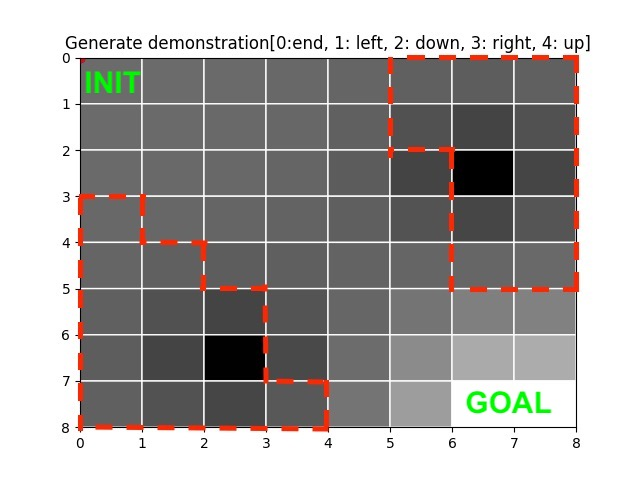
\includegraphics[width=1.\linewidth]{sec3_2.jpg}
	   \label{fig:sec3_2}
	\end{minipage}\hfill
}
\subfigure[]{
	\begin{minipage}[c][1\width]{
	   0.4\textwidth}
	   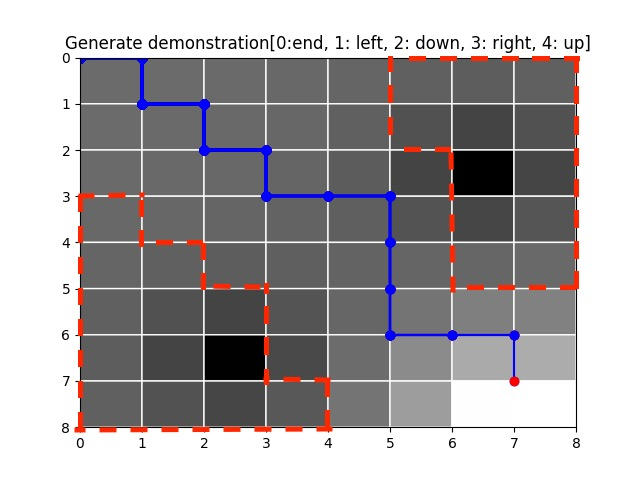
\includegraphics[width=1.\linewidth]{sec3_3.jpg}
	   \label{fig:sec3_3}
	\end{minipage}\hfill
}
\subfigure[]{
	\begin{minipage}[c][1\width]{
	   0.4\textwidth}
	   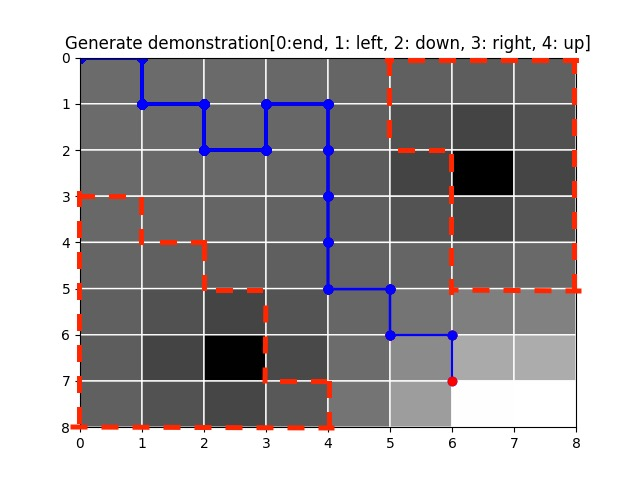
\includegraphics[width=1.\linewidth]{sec3_4.jpg}
	   \label{fig:sec3_4}
	\end{minipage}\hfill
}
\subfigure[]{
	\begin{minipage}[c][1\width]{
	   0.4\textwidth}
	   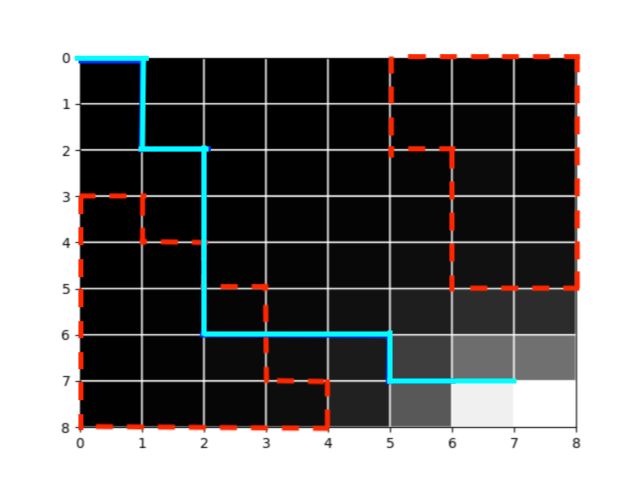
\includegraphics[width=1.\linewidth]{sec3_5.png}
	   \label{fig:sec3_5}
	\end{minipage}\hspace{0.012\linewidth}
}
\caption[Navigation task in gridworld]{
(a) The 8 x 8 gridworld. Lighter grid cells indicate relatively higher rewards while darker ones indicate lower rewards. It is regarded by the expert that the two black grid cells have the lowest rewards, while the two white ones constituting the goal area have the the highest rewards. The grid cells enclosed by red dashed lines are labelled as unsafe. (b) The blue line is the first representative trajectory that expert perform during demonstration. (c) The blue line is the second representative trajectory that expert perform during demonstration. (d) The rewards of the goal states have very high contrast against all other states. The difference between unsafe states and nearby states is so small that the agent has a high probability of performing a trajectory passing through the unsafe states as indicated by the cyan line.
}
\label{fig:grid_world1}
\end{figure}
%\vspace{-3mm}

We use a 8 x 8 grid world navigation example as shown in Fig.~\ref{fig:grid_world1} to illustrate this problem. The agent starts from the upper-left corner and moves from cell to cell until reaching the lower-right corner or a maximal step length $t<64$. Meanwhile, there are several cells labelled as unsafe enclosed by the red dashed lines shown near the upper-right and lower-left corners. These are regions that agent should avoid. 
In each time step, the agent can choose to stay in current cell or move to an adjacent cell. Due to stochasticity of the system, it has $30\%$ chance of moving randomly instead of moving accroding its decision. 
The expert knows the goal area, the unsafe area and the reward mapping on all states as shown in Fig.~\ref{fig:sec3_2}. For each state $s\in S$, the feature vector $f(s)$ consists of $4$ feature functions $f_i(s),\ i = 0, 1, 2, 3$. All of them are radial basis functions which respectively depend on the squared Euclidean distances between $s$ and the $4$ states with the highest or lowest rewards as shown in Fig.~\ref{fig:sec3_2}. In addition, a specification $\Phi$ formalized in PCTL is given to capture the safety requirement. In Eq.~\ref{eq:example-spec}, $p^*$ is the upper bound of the probability of reaching an unsafe state within $t=64$ steps and can be set by any value in $[0, 1]$ initially.
\begin{equation}
\Phi ::= P_{=?|s_0}[\true\ \until^{\leq t}\ \texttt{unsafe}]\leq p^*
\label{eq:example-spec}
\end{equation}

We extend the satisfaction relation $\models$ in PCTL and define that a policy $\pi\models\Phi$ if the initial state $s_0$ of DTMC $M_\pi$ induced from MDP $M$ by policy $\pi$ satisfies the PCTL property in $\Phi$, then $\pi\models\Phi$. define the satisfaction relation $\models$ between a policy $\pi$ and a safety specification $\Phi$ as . We illustrate two scenarios in this simple example. The first simulates a setting with abundant expert demonstrations, i.e. $\mu_E$ is directly generated from the optimal policy $\pi_E$ with respect to the predetermined $\omega_E$ which results in the reward mapping in Fig.~\ref{fig:sec3_2}. In this case, the AL algorithm can accurately recover $\pi_E$. 
Model checking result shows that the probability of reaching an unsafe state by following the learnt policy, or the expert policy $\pi_E$ itself, is $11.7\%$. Hence, the specification is satisfied in this scenario. In the second scenario, which is more realistic, the expert follows $\pi_E$ but only performs a limited number of demonstrations which are all successful and safe. As indicated by the two representative (in blue) trajectories shown in Fig.~\ref{fig:sec3_3} and Fig.~\ref{fig:sec3_4}, $10,000$\footnote{This number is actually considered small for the size of this problem.} trajectories were used as expert demonstrations. 
The reward function that induces the learnt policy in this scenario is shown in Fig.~{\ref{fig:sec3_5}}.
Observe that only the goal area has been learnt whereas the agent is oblivious to the unsafe regions (treating them in the same way as other black cells). Indeed, probability of reaching an unsafe state within $64$ steps with this policy turns out to be $98\%$ (thus violating the safety requirement by a large margin).  
To make matters worse, the value of $p^*$ may be decided or revised after a policy has been learnt. In that case, even the original expert policy $\pi_E$ is unsafe, e.g., when $p^*=10\%$. 
Thus, we need to adapt the AL algorithm to account for this additional safety requirement. 
\begin{definition}
\textbf{The safety-aware apprenticeship learning (SafeAL) problem} is, given an $MDP\backslash R$, a set of $m$ trajectories $\{\tau_0, \tau_1, ..., \tau_{m-1}\}$ demonstrated by an expert, and a specification $\Phi$, to learn a policy $\pi$ that satisfies $\Phi$ and is $\epsilon$-close to the expert policy $\pi_E$.
\end{definition}


\section{A Framework for Safety-Aware Learning}
\label{sec:section4}
\graphicspath{{2_Body/section4/figures/}}
%\section{Counterexample-Guided Inductive Learning }
%%\vspace{-2mm}
\begin{figure}
\centering
  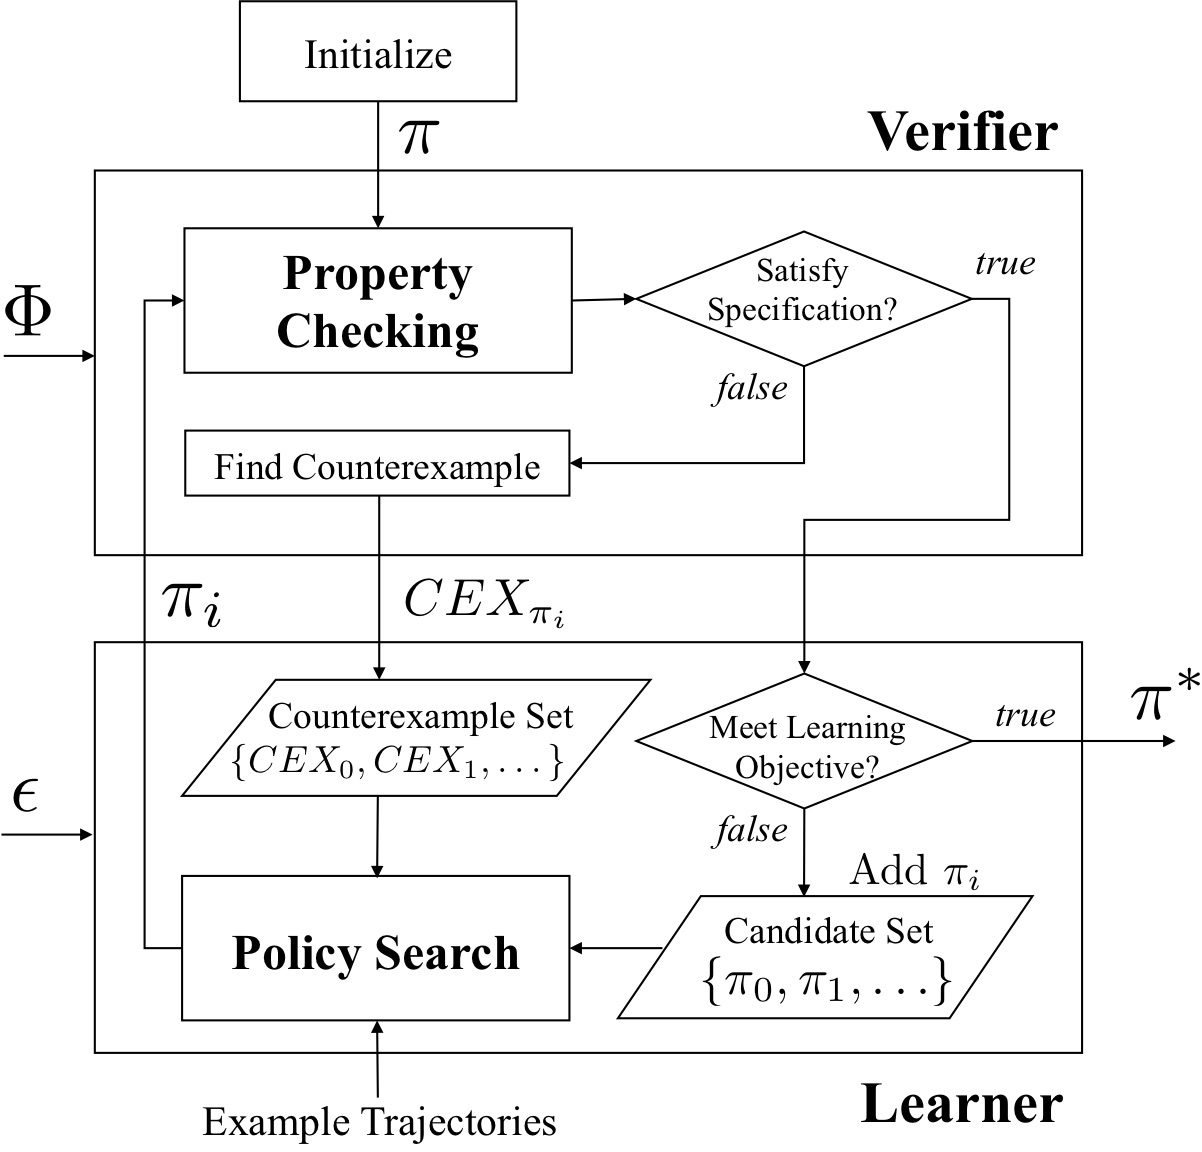
\includegraphics[width=12cm, height=12cm]{overview.jpg}
  %\vspace{-2mm}
\caption[Counterexample-Guided Apprenticeship Learning]{
Our safety-aware learning framework. Given an initial policy $\pi_0$, a specification $\Phi$ and a learning objective (as captured by $\epsilon$), the framework iterates between a {\it verifier} and a {\it learner} to search for a policy $\pi^*$ that satisfies both $\Phi$ and $\epsilon$. One invariant that this framework maintains is that all the $\pi_i$'s in the candidate policy set satisfy $\Phi$.}
\label{fig:sec4_1}
\end{figure}
In this section, we describe a general framework for safety-aware learning. 
This novel framework utilizes information from both the expert demonstrations and a verifier. 
The proposed framework is illustrated in Fig.~\ref{fig:sec4_1}. Similar to the \emph{counterexample-guided inductive synthesis} (CEGIS) paradigm~\cite{CEGIS}, our framework consists of a {\it verifier} and a {\it learner}. The verifier checks if a candidate policy satisfies the safety specification $\Phi$. In case $\Phi$ is not satisfied, the verifier generates a counterexample for $\Phi$. 
The main difference from CEGIS is that our framework considers not only functional correctness, e.g., safety, but also performance (as captured by the learning objective). Starting from an initial policy $\pi_0$, each time the learner learns a new policy, the verifier checks if the specification is satisfied. If true, then this policy is added to the candidate set, otherwise the verifier will generate a (minimal) counterexample and add it to the counterexample set. During the learning phase, the learner uses both the counterexample set and candidate set to find a policy that is close to the (unknown) expert policy and far away from the counterexamples. The goal is to find a policy that is $\epsilon$-close to the expert policy and satisfies the specification. 
 %Observe that the goal area and the unsafe regions are now well represented as in the ground-truth reward.
%\vspace{-3mm}

%\vspace{-8mm}
\begin{figure}[h]
\centering
\subfigure[]{
	\hspace{0.1\linewidth}\begin{minipage}[c][1\width]{
	   0.4\textwidth}
	   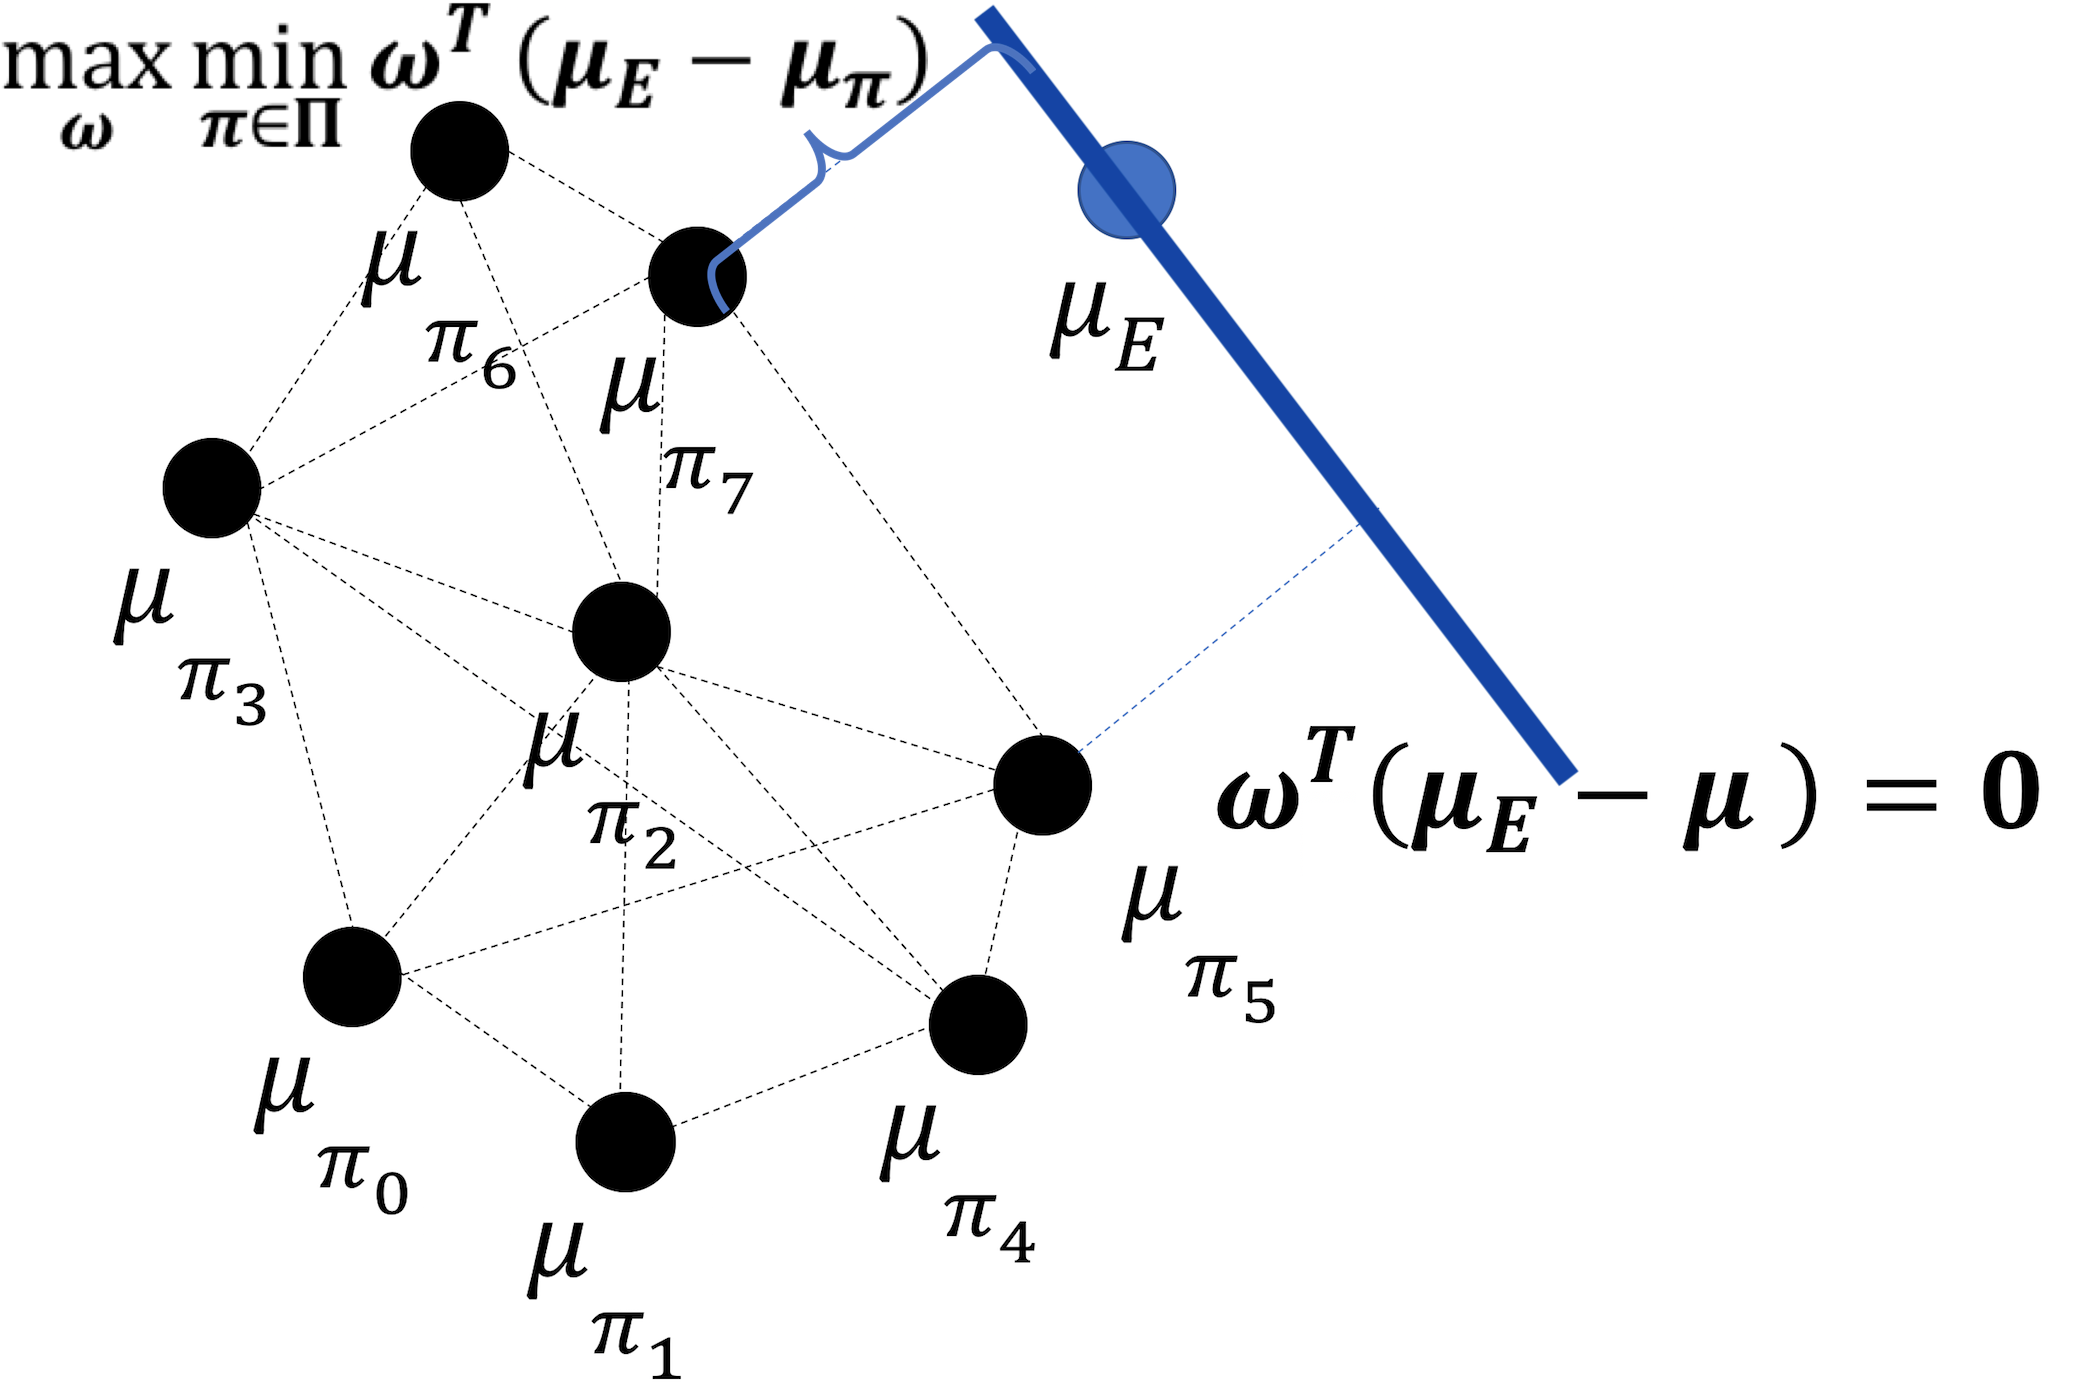
\includegraphics[width=1.3\linewidth]{sec4_4.png}
	   \label{fig:sec4_2}
	\end{minipage}\hspace{0.2\linewidth}
}
\subfigure[]{
	\begin{minipage}[c][1\width]{
	   0.4\textwidth}
	   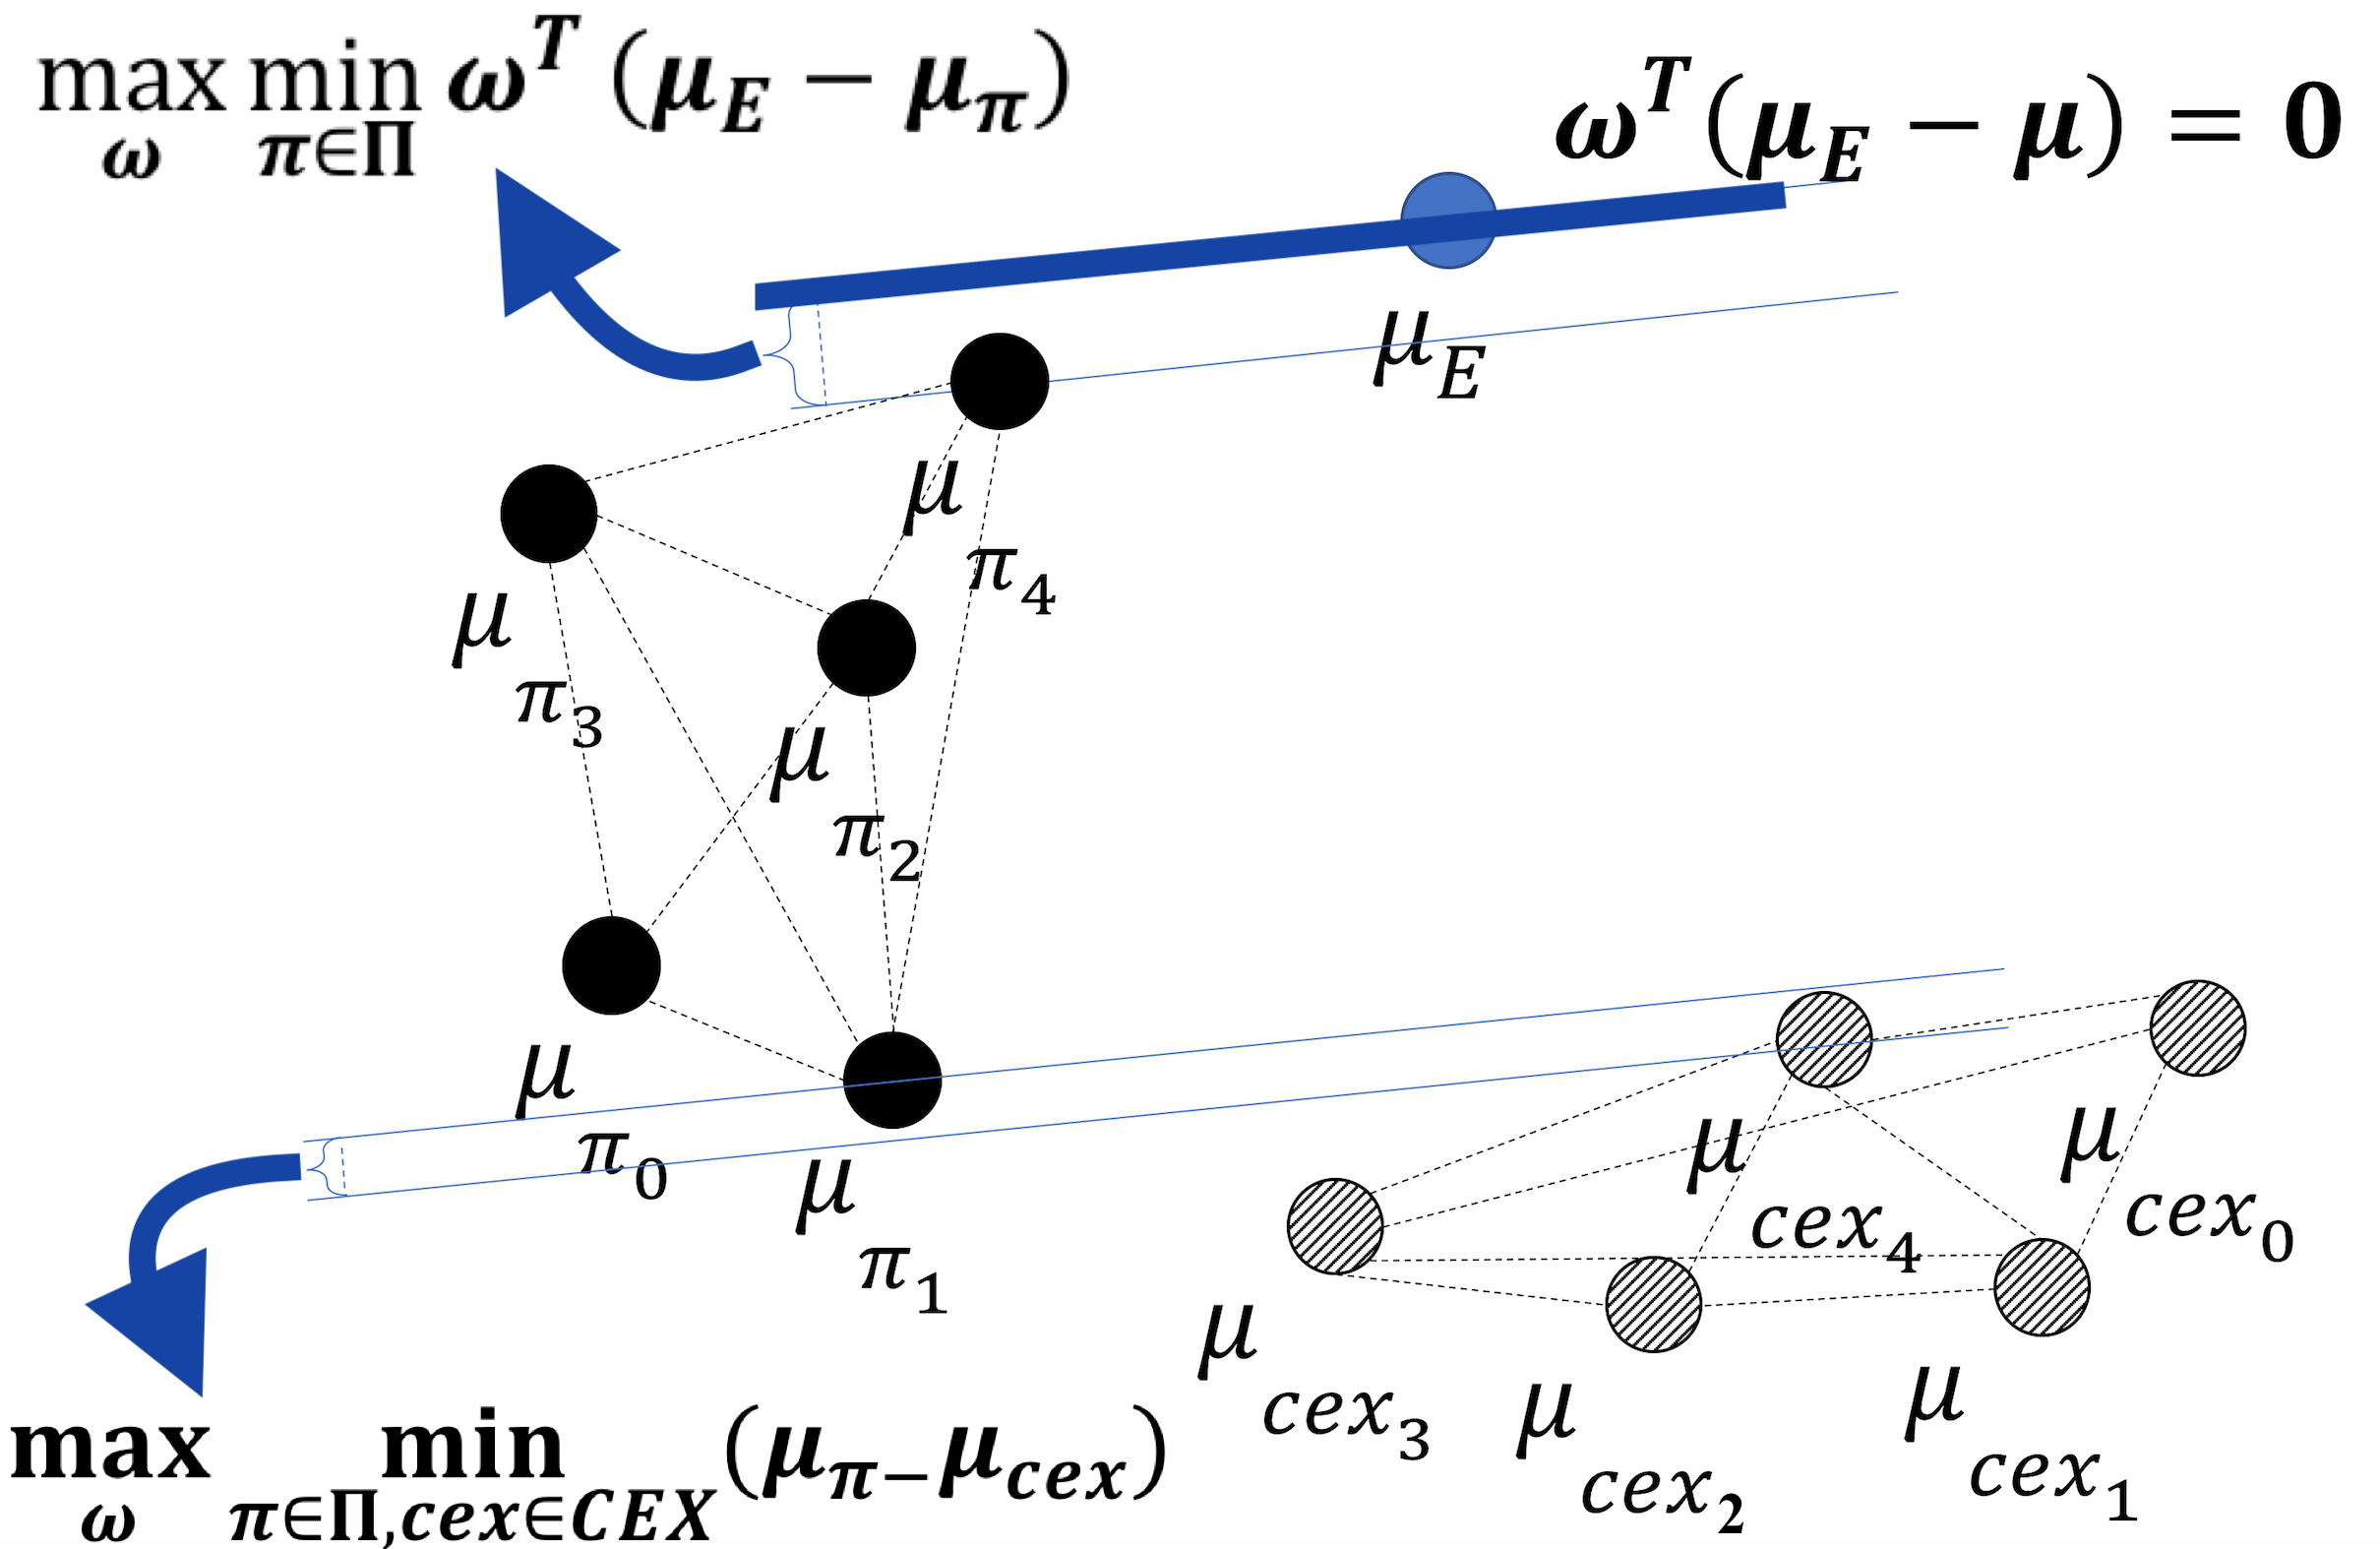
\includegraphics[width=1.3\linewidth]{sec4_3.png}
	   \label{fig:sec4_3}
	\end{minipage}\hspace{0.1\linewidth}
}
%\vspace{-3mm} 
\caption[Max margin principle]{(a) Learn from expert. (b) Learn from both expert demonstrations and counterexamples.}
%\vspace{-4mm}
\end{figure}
%%\vspace{-5mm} we 

Learning from a (minimal) counterexample $cex_{\pi}$ of a policy $\pi$ is similar to learning from expert demonstrations. %since they are both trajectories generated by their corresponding policies. 
The basic principle of the AL algorithm proposed in \cite{Abbeel:2004:ALV:1015330.1015430} is to find a weight vector $\omega$ under which the expected reward of $\pi_E$ maximally outperforms any mixture of the policies in the candidate policy set $\Pi=\{\pi_0, \pi_1, \pi_2, \ldots\}$. Thus, $\omega$ can be viewed as the normal vector of the hyperplane $\omega^T(\mu - \mu_E) = 0$ that has the maximal distance to the convex hull of the set $\{\mu_{\pi}\:|\:\pi\in\Pi\}$ as illustrated in the 2D feature space in Fig.~\ref{fig:sec4_2}. 
It can be shown that $\omega^T \mu_\pi \geq \omega^T \mu_{\pi'}$ for all previously found $\pi'$s. Intuitively, this moves the candidate $\mu_\pi$ closer to $\mu_E$.
Similarly, we can apply the same max-margin separation principle to maximize the distance between the candidate policies and the counterexamples (in the $\mu$ space).     
Let ${CEX}= \{cex_0, cex_1, cex_2, ...\}$ denote the set of counterexamples of the policies that do not satisfy the specification $\Phi$. 
Maximizing the distance between the convex hulls of the sets $\{\mu_{cex}\:|\:cex\in{CEX}\}$ and $\{\mu_{\pi}\:|\:\pi\in\Pi\}$ is equivalent to maximizing the distance between the parallel supporting hyperplanes of the two convex hulls as shown in Fig.~\ref{fig:sec4_3}. The corresponding optimization function is given in Eq.~(\ref{eq:sec4_2}).
%\footnote{The last state of a counterexample trajectory $\tau\in CEX_{\pi}$ is regarded as absorbing when calculating the expected features of this trajectory in order to amplify the significance of features of the unsafe state. The expected feature counts of all the counterexample trajectories are also normalized by the sum of their probabilities.}.
%\vspace{-2mm}
\begin{equation}
\delta = \max\limits_{\omega}\min\limits_{\pi\in\Pi, cex\in CEX}\ \omega^T(\mu_{\pi}-\mu_{cex})\label{eq:sec4_2}\qquad s.t.\:||\omega||_2\leq 1
\end{equation}
%\vspace{-2mm}

To attain good performance similar to that of the expert, agent still needs to learn from $\mu_E$. Thus, the overall problem can be formulated as a multi-objective optimization problem that combines (\ref{eq:sec1_1}) and (\ref{eq:sec4_2}) into (\ref{eq:sec4_3}).
%\vspace{-3mm}
\begin{equation}
\max\limits_\omega \min\limits_{\pi \in \Pi, \tilde\pi \in \Pi, cex \in CEX} (\omega^T (\mu_E - \mu_{\pi}),\ \omega^T (\mu_{\tilde\pi} - \mu_{cex}) )\qquad s.t.\:||\omega||_2\leq 1
\label{eq:sec4_3}
\end{equation}
%\vspace{-5mm}


\section{An Algorithm for Counterexample-Guided Apprenticeship Learning}
\label{sec:section5}
\graphicspath{{2_Body/section5/figures/}}
%\section{Safety-aware apprenticeship learning algorithm}
%%\vspace{-2mm}
In this section, we introduce the Counterexample Guided Apprenticeship Learning (CEGAL)
algorithm to solve the SafeAL problem. 
It can be viewed as a special case of the safety-aware learning framework described in the previous section. 
In addition to combining policy verification, counterexample generation and AL, our approach uses an adaptive weighting scheme to weight the separation from $\mu_E$ with the separation from $\mu_{cex}$.
%\vspace{-4mm}
\begin{eqnarray}
&&\underset{\omega}{\max}\underset{\pi\in\Pi_S,\tilde{\pi}\in\Pi_S, cex\in CEX}{\min}\ \omega^T(k(\mu_E - \mu_{\pi})+(1-k)(\mu_{ \tilde{\pi}}  - \mu_{cex}))\label{eq:sec5_1}\\
&&s.t.\: ||\omega||_2\leq 1 \label{eq:sec5_4},\: k\in[0, 1]\label{eq:sec5_5} \nonumber\\ 
&&\quad\ \:\omega^T(\mu_E - \mu_{\pi})\leq\omega^T(\mu_E - \mu_{\pi'}),\ \forall\pi'\in\Pi_S \label{eq:sec5_2} \nonumber\\ 
&&\quad\ \:\omega^T(\mu_{\tilde{\pi}} - \mu_{cex})\leq\omega^T(\mu_{ \tilde{\pi}'} - \mu_{cex'}),\ \forall \tilde{\pi}'\in\Pi_S, \forall cex'\in{CEX} \nonumber
\end{eqnarray}
%\vspace{-3mm}
In essence, we take a weighted-sum approach for solving the multi-objective optimization problem  (\ref{eq:sec4_3}). Assuming that $\Pi_S=\{\pi_{1},$ $\pi_{2},$ $\pi_{3},$ $\ldots \}$ is a set of candidate policies that all satisfy $\Phi$, ${CEX} =\{cex_1,$ $cex_2,$ $cex_3,$ $\ldots\}$ is a set of counterexamples. We introduce a parameter $k$ and change (\ref{eq:sec4_3}) into a weighted sum optimization problem (\ref{eq:sec5_1}). Note that $\pi$ and $\tilde\pi$ can be different. The optimal $\omega$ solved from (\ref{eq:sec5_1}) can be used to generate a new policy $\pi_\omega$ by using algorithms such as policy iteration. 
We use a probabilistic model checker, such as PRISM~\cite{kwiatkowska2002prism}, to check if $\pi_\omega$ satisfies $\Phi$. If it does, then it will be added to $\Pi_S$. Otherwise, a counterexample generator, such as COMICS~\cite{DBLP:journals/corr/abs-1206-0603}, is used to generate a (minimal) counterexample $cex_{\pi_\omega}$, which will be added to ${CEX}$.  

%\vspace{-2mm}
\begin{algorithm}[htb]
\caption{Counterexample-Guided Apprenticeship Learning (CEGAL)}
\begin{algorithmic}[1]
\State \textbf{Input}:
\\\qquad $M\gets$ A partially known $MDP\backslash R$; $f\gets$ A vector of feature functions
\\\qquad $\mu_E\gets$ The expected features of expert trajectories $\{\tau_0, \tau_1, \ldots,\tau_m\}$
\\\qquad $\Phi\gets$ Specification; $\epsilon\gets$ Error bound for the expected features;
\\\qquad $\sigma, \alpha\in(0, 1)\gets$ Error bound $\sigma$ and step length $\alpha$ for the parameter $k$; 
\State \textbf{Initialization}:
\\\qquad $inf\leftarrow0, sup\leftarrow1, k\leftarrow sup$ \Comment{Initialize multi-optimization parameter $k$}
\\\qquad $\Pi_S\leftarrow\{\pi_0\}$ \Comment{Initialize candidate set with an \textbf{initial safe policy}}
\\\qquad $CEX\leftarrow\emptyset$ \Comment{Initialize counterexample set as empty}
\\\qquad $\pi_1\leftarrow$ Policy learnt from $\mu_E$ via apprenticeship learning
\State \textbf{Iteration $i\ (i\geq 1)$}:
\\\qquad\textbf{Verifier:}
\\\qquad\qquad status $\gets Model\_Checker(M,\pi_i, \Phi)$
\\\qquad\qquad \textbf{If} status = SAT, \textbf{then go to Learner}
\\\qquad\qquad \textbf{If} status = UNSAT
\\\qquad\qquad\qquad $cex_{\pi_i}\gets Counterexample\_Generator(M,\pi_i,\Phi)$
\\\qquad\qquad\qquad Add $cex_{\pi_i}$ to $CEX$ and solve $\mu_{cex_{\pi_i}}$, \textbf{go to Learner} 
\\\qquad\textbf{Learner:}
\\\qquad\qquad \textbf{If} status = SAT
\\\qquad\qquad\qquad \textbf{If} $||\mu_E-\mu_{\pi_i}||_2\leq \epsilon$, {\bf then return} $\pi_i$
\\\Comment{Converge. $\pi_i$ is {$\epsilon$-close} to $\pi_E$}
\\\qquad\qquad\qquad Add $\pi_i$ to $\Pi_S$, $inf \leftarrow k, k \leftarrow sup$\Comment{Update $\Pi_S$, $inf$ and reset $k$}
\\\qquad\qquad \textbf{If} status = UNSAT
\\\qquad\qquad\qquad \textbf{If} $|k - inf|\leq\sigma$, {\bf then return} $\pi^*\leftarrow\underset{{\pi}\in \Pi_S}{argmin}||\mu_E - \mu_{{\pi}}||_2$\\\Comment{Converge. $k$ is too close to its lower bound. }
\\\qquad\qquad\qquad $k \leftarrow \alpha\cdot inf + (1 - \alpha)k$ 
\Comment{Decrease k to learn for safety}
\\\qquad\qquad $\omega_{i+1} \leftarrow arg\underset{\omega}{max}\underset{\pi\in\Pi_S, \tilde{\pi}\in\Pi_S, cex\in CEX}{\min}\ \omega^T(k(\mu_E - \mu_{\pi})+(1-k)(\mu_{\tilde{\pi}}  - \mu_{cex}))$
\\\Comment{Note that the multi-objective optimization function recovers AL when $k=1$} 
\\\qquad\qquad $\pi_{i+1}, \mu_{\pi_{i+1}}\gets$ Compute the optimal policy $\pi_{i+1}$ and its expected features $\mu_{\pi_{i+1}}$ for the MDP $M$ with reward $R(s)=\omega_{i+1}^T f(s)$
\\\qquad{\bf Go to next iteration}
\end{algorithmic}
\label{algo1}
\end{algorithm}

Algorithm 1 describes CEGAL in detail. 
With a constant $sup=1$ and a variable $inf\in[0, sup]$ for the upper and lower bounds respectively, the learner determines the value of $k$ within $[inf, sup]$ in each iteration depending on the outcome of the verifier and uses $k$ in solving (\ref{eq:sec5_1}) in line 27. 
Like most nonlinear optimization algorithms, this algorithm requires an initial guess, which is an initial safe policy $\pi_0$ to make $\Pi_S$ nonempty. A good initial candidate would be the maximally safe policy for example obtained using PRISM-games~{\cite{Kwiatkowska2017}}. 
Without loss of generality, we assume this policy satisfies $\Phi$.
%Given the PCTL formula $\psi$ used in $\Phi$, such as $\psi::=\true\ \until^{\leq t}\ \texttt{unsafe}$ in (\ref{eq:example-spec}), PRISM-games solves $min~P_{=?}[\psi]$ and returns a \textcolor{red}{safest} policy that satisfies the minimization. 
%If the policy satisfies $\Phi$, then $\Phi$ is proved to be satisfiable and the policy can be used as $\pi_0$ to start the iteration. 
Suppose in iteration $i$, an intermediate policy $\pi_i$ learnt by the learner in iteration $i-1$ is verified to satisfy $\Phi$, then we increase $inf$ to $inf=k$ and reset $k$ to $k=sup$ as shown in line 22. 
If $\pi_i$ does not satisfy $\Phi$, then we reduce $k$ to $k=\alpha\cdot inf + (1 - \alpha)k$  as shown in line 26 where $\alpha\in(0, 1)$ is a step length parameter. 
If $|k-inf|\leq\sigma$ and $\pi_i$ still does not satisfy $\Phi$, the algorithm chooses from $\Pi_S$ a best safe policy $\pi^*$ which has the smallest margin to $\pi_E$ as shown in line 24. If $\pi_i$ satisfies $\Phi$ and is {$\epsilon$-close} to $\pi_E$, the algorithm outputs $\pi_i$ as show in line 19. For the occasions when $\pi_i$ satisfies $\Phi$ and $inf = sup = k = 1$, solving (\ref{eq:sec5_1}) is equivalent to solving (\ref{eq:sec1_1}) as in the original AL algorithm.

\begin{remark}
The initial policy $\pi_0$ does not have to be maximally safe, although such a policy can be used to verify if $\Phi$ is  satisfiable at all. 
Naively safe policies often suffice for obtaining a safe and performant output at the end. Such a policy can be obtained easily in many settings, e.g., in the grid-world example one safe policy is simply staying in the initial cell. 
In both cases, $\pi_0$ typically has very low performance since satisfying $\Phi$ is the only requirement for it. An initial safe policy can also be generated (with no guarantee) by solving (\ref{eq:sec4_2}) iteratively as shown in Algorithm 2.
%We also note that apprenticeship learning itself does not guarantee safety for the final output even if we initialize it with a safe policy.   
\end{remark}

%%\vspace{-4mm}
\begin{algorithm}[htb]
\caption{Initial Safe Policy Generation}
\begin{algorithmic}[1]
%\State \textbf{Input}:
%\\\qquad$M \gets$ MDP model
%\\\qquad$\mu_E\gets$ Expert's expected features; $\Phi\gets$ specification; $\epsilon\gets$ error bound.
%\\\qquad$\Pi_{CEX}=\{\}$\Comment{Counterexample set initialized to be an empty set}
%\\\qquad$\pi^*=Null\gets$ Policy to be output, preset to be Null
%\\\qquad$\mu^*=Null\gets$ Expected feature of $\pi^*$, preset to be Null
%\\\qquad ${CEX}=\emptyset \gets$ Set of counterexample features
%\\\qquad $\Pi_{S}=\emptyset \gets$ Set of safe policy features
%\\\qquad $\Pi=\emptyset \gets$ Set of policy features
%\\\qquad $SafePolicyGen() \gets$ Safe policy generator
%\\\qquad\qquad
\State \textbf{Initialize}: 
\\\qquad$\pi_0\gets$Any arbitrary policy  \Comment{Can be any policy, e.g. the policy learnt via AL}  
\\\qquad$\epsilon\gets$ Error bound for the expected features
\\\qquad$CEX\gets\emptyset$
%\\\qquad\qquad
\State \textbf{Iteration}: 
\\\qquad In iteration $i\geq1$, get $\pi_i$ from last iteration
\\\qquad\textbf{Verifier:}
\\\qquad\qquad status $\gets Model\_Checker(M,\pi_i, \Phi)$
\\\qquad\qquad \textbf{If} status = SAT, \textbf{then go to Learner}
\\\qquad\qquad \textbf{If} status = UNSAT
\\\qquad\qquad\qquad $cex_{\pi_i}\gets Counterexample\_Generator(M,\pi_i,\Phi)$
\\\qquad\qquad\qquad Add $cex_{\pi_i}$ to $CEX$ and solve $\mu_{cex_{\pi_i}}$, \textbf{go to Learner} 
\\\qquad\textbf{Learner:}
\\\qquad\qquad \textbf{If} status = SAT
\\\qquad\qquad\qquad Return $\pi_i$\Comment{End iteration once a safe policy is found}
\\\qquad\qquad \textbf{If} status = UNSAT
\\\qquad\qquad\qquad \textbf{If} $|CEX|>1$ and $\|\frac{\underset{cex \in |CEX|}{\sum}\mu_{cex}\ \ }{|CEX|}-\frac{\mu_{cex_i} + \underset{cex \in |CEX|}{\sum}\mu_{cex}\ \ }{1 + |CEX|}\|_2\leq\epsilon$
\\\qquad\qquad\qquad\qquad  \textbf{Then} return Null\\\Comment{Fail to find a safe policy since adding a new counterexample hardly changes the centroid of existing counterexample cluster.}
%\\\qquad\qquad $\omega_{i+1} = \underset{\omega}{argmax} \underset{\mu\in \Pi_{CEX}}{min}\ (-\omega^T\mu)$
\\\qquad\qquad $\omega_{i+1} = arg\max_{\omega} \min_{cex\in CEX}\ (-\omega^T\mu_{cex})$
\\\qquad\qquad $\pi_{i+1}\gets$ Optimal policy of $\omega_{i+1}$

\\\qquad Go to next iteration

\end{algorithmic}
\end{algorithm}
%%\vspace{-4mm}

\begin{theorem}
%If the initial policy $\pi_0$ satisfies $\Phi$, then Algorithm~\ref{algo1} is guaranteed to output a policy $\pi^*$, such that (1) $\pi^*$ satisfies $\Phi$, and (2) the margin between the expected features $ \mu_{\pi^*}$ of $\pi^*$ and the expert's features $\mu_E$ has no smaller margin to expert's features $\mu_E$ than the expected features $\mu_{\pi_0}$ of the initial policy $\pi_0$, i.e. $\|\mu_E - \mu_{\pi^*}\|_2\leq\|\mu_E - \mu_{\pi_0}\|_2$. 
Given an initial policy $\pi_0$ that satisfies $\Phi$, Algorithm~\ref{algo1} is guaranteed to output a policy $\pi^*$, such that (1) $\pi^*$ satisfies $\Phi$, and 
(2) the performance of $\pi^*$ is at least as good as that of $\pi_0$ when compared to $\pi_E$, i.e. $\|\mu_E - \mu_{\pi^*}\|_2\leq\|\mu_E - \mu_{\pi_0}\|_2$. 
\end{theorem}
\noindent{\it Proof sketch. }%\revise{???}
The first part of the guarantee can be proven by case splitting. 
Algorithm~\ref{algo1} outputs $\pi^*$ either when $\pi^*$ satisfies $\Phi$ and is {$\epsilon$-close} to $\pi_E$, or when $|k-inf|\leq \sigma$ in some iteration. 
In the first case, $\pi^*$ clearly satisfies $\Phi$. 
In the second case, $\pi^*$ is selected from the set $\Pi_S$ which contains all the policies that have been found to satisfy $\Phi$ so far, so $\pi^*$ satisfies $\Phi$.
For the second part of the guarantee, the initial policy $\pi_0$ is the final output $\pi^*$ if $\pi_0$ satisfies $\Phi$ and is {$\epsilon$-close} to $\pi_E$. 
Otherwise, $\pi_0$ is added to $\Pi_S$ if it satisfies $\Phi$.  
During the iteration, if $|k-inf|\leq \sigma$ in some iteration, then the final output is $\pi^*=\underset{{\pi}\in\Pi_S}{argmin}||\mu_E - \mu_{{\pi}}||_2$, so it must satisfy $\|\mu_E -  \mu_{\pi^*}\|_2\leq\|\mu_E - \mu_{\pi_0}\|_2$. 
If a learnt policy $\pi^*$ satisfies $\Phi$ and is {$\epsilon$-close} to $\pi_E$, then Algorithm~\ref{algo1} outputs $\pi^*$ without adding it to $\Pi_S$. Obviously $\|\mu_E - \mu_{{\pi}}\|_2>\epsilon, \forall{\pi}\in\Pi_S$, so $\|\mu_E -  \mu_{\pi^*}\|_2\leq\|\mu_E - \mu_{\pi_0}\|_2$.

\noindent
{\it Discussion.} In the worst case CEGAL will return the initial safe policy. However, this can be because a policy that simultaneously satisfies $\Phi$ and is $\epsilon$-close to the expert's demonstrations does not exist. Comparing to AL which offers no safety guarantee and finding the maximally safe policy which has very poor performance, CEGAL provides a principled way of guaranteeing safety while retaining performance.

\noindent


\section{Convergence}
\label{sec:section6}
\graphicspath{{2_Body/section6/figures/}}

Algorithm 1 is guaranteed to converge. Let $inf_t$ be the $t^{th}$ assigned value of $inf$. After $inf_t$ is given, $k$ is decreased from $k_0=sup$ iteratively by $k_{i}=\alpha\cdot inf_t + (1 - \alpha)k_{i-1}$ until either $|k_i-inf_t|\leq \sigma$ in line 24 or a new safe policy is found in line 18. The update of $k$ satisfies the following equality.
%\vspace{-3mm}
\begin{eqnarray}
\frac{|k_{i+1} - inf_t|}{|k_i - inf_t|}&=& \frac{\alpha\cdot inf_t + (1 - \alpha)k_i - inf_t}{k_i - inf_t} =  1-\alpha
%&=& \frac{k_{i+1} - k^*}{k_i - k^*}\\
\end{eqnarray}
%\vspace{-3mm}

Thus, it takes no more than 1+$\log_{1-\alpha}\frac{\sigma}{sup - inf_t}$ iterations for either the algorithm to converge in line 24 or a new safe policy to be found in line 18. If a new safe policy is found in line 18, $inf$ will be assigned in line 22 by the current value of $k$ as $inf_{t+1}=k$ which obviously satisfies $inf_{t+1} - inf_t \geq(1-\alpha)\sigma$. After the assignment of $inf_{t+1}$, the iterative update of $k$ resumes. Since $sup-inf_t \leq 1$, the following inequality holds.
%\vspace{-3mm}
\begin{eqnarray}
\frac{|inf_{t+1} - sup|}{|inf_{t} - sup|}&\leq&\frac{sup -inf_{t} - (1-\alpha)\sigma}{sup- inf_{t}}\leq 1 - (1-\alpha)\sigma
\end{eqnarray}
%\vspace{-3mm}

Obviously, starting from an initial $inf=inf_0<sup$, with the alternating update of $inf$ and $k$, $inf$ will keep getting close to $sup$ unless the algorithm converges as in line 24 or a safe policy {$\epsilon$-close} to $\pi_E$ is found as in line 19. The extreme case is that finally $inf=sup$ after no more than $\frac{sup-inf_0}{(1-\alpha)\sigma}$ updates on $inf$. Then, the problem becomes AL. Therefore, the worst case of this algorithm can have two phases. In the first phase, $inf$ increases from $inf=0$ to $inf=sup$. Between each two consecutive updates $(t, t+1)$ on $inf$, there are no more than $\log_{1-\alpha}\frac{(1-\alpha)\sigma}{sup - inf_t}$ updates on $k$ before $inf$ is increased from $inf_t$ to $inf_{t+1}$. Overall, this phase takes no more than
%\vspace{-3mm}
\begin{equation}
{\underset{0\leq i< \frac{sup-inf_0}{(1-\alpha)\sigma}}{\sum}\log_{1-\alpha} \frac{(1-\alpha)\sigma}{sup-inf_0-i\cdot (1-\alpha)\sigma}} = {\underset{0\leq i< \frac{1}{(1-\alpha)\sigma}}{\sum}\log_{1-\alpha} \frac{(1-\alpha)\sigma}{1-i\cdot (1-\alpha)\sigma}}
\end{equation}
%\vspace{-3mm}

\noindent iterations to reduce the multi-objective optimization problem to original apprenticeship learning and then the second phase begins. Since $k=sup$, the iteration will stop immediately when an unsafe policy is learnt as in line 24. This phase will not take more iterations than original AL algorithm does to converge.

The convergence analysis of AL can be found in~\cite{Abbeel:2004:ALV:1015330.1015430}. First it's assumed that the ball with radius $\epsilon$ around $\mu_E$, which is a set $\{\mu\mid d(\mu_E, \mu)\leq\epsilon\}$, will have intersection with be the convex hull of the set of feature expectations of candidate policy set $\Pi$ after $n$ iterations. Then it's provable that $n$ satisfies
\begin{equation}
n\leq O\big(\frac{k}{(1-\gamma)^2\epsilon^2}\log{\frac{k}{(1-\gamma)\epsilon}}\big)
\end{equation}
where $k$ is the number of features, $\gamma$ is the discount factor. It's also ensured in~\cite{Abbeel:2004:ALV:1015330.1015430} that the number of sample demonstrations needed to make AL algorithm output with probability at least $1-\delta$ should suffice that
\begin{equation}
m\geq \frac{2k}{(1-\gamma)^2\epsilon^2}\log{\frac{2k}{\delta}}
\end{equation}

In each iteration of Algorithm 1, the algorithm first solves a second-order cone programming (SOCP) problem (\ref{eq:sec5_1}) to learn a policy. SOCP problems can be solved in polynomial time by interior-point (IP) methods~\cite{Kuo:2004aa}.
PCTL model checking for DTMCs can be solved in time linear in the size of the formula and polynomial in the size of the state space~\cite{Hansson1994}. 
Counterexample generation can be done either by enumerating paths using the $k$-shortest path algorithm or determining a critical subsystem using either a $SMT$ formulation or mixed integer linear programming (MILP)~\cite{Wimmer2012}. For the $k$-shortest path-based algorithm, it can be computationally expensive sometimes to enumerate a large amount of paths (i.e. a large $k$) when $p^*$ is large. This can be alleviated by using a smaller $p^*$ during calculation, which is equivalent to considering only paths that have high probabilities.
%\vspace{-1mm}


\chapter{Experiments}
\label{sec:exp}
\graphicspath{{2_Body/experiments/figures/}}
%\vspace{-1mm}
We evaluate our algorithm on three case studies: (1) grid-world, (2) cart-pole, and (3) mountain-car. The cart-pole environment\footnote{\url{https://github.com/openai/gym/wiki/CartPole-v0}} and the mountain-car environment\footnote{\url{https://github.com/openai/gym/wiki/MountainCar-v0}} are obtained from OpenAI Gym. All experiments are carried out on a quad-core i7-7700K processor running at 3.6 GHz with 16 GB of memory. 
Our prototype tool was implemented in Python\footnote{\url{https://github.com/zwc662/CAV2018}}.
For the OpenAI-gym experiments, in each step, the agent sends an action to the OpenAI environment and the environment returns an observation and reward. 
The parameters are $\gamma=0.99, \sigma=10^{-5}, \alpha=0.5$. For grid-world, $\epsilon=1E-5$, whereas for OpenAI-gym environments, $\epsilon=10$.
We use model checking results to show that our algorithm can guarantee the safety of the learnt policy. Moreover, we quantitatively show that the learnt policy has comparable performance compared with the one directly learnt using AL.
%\vspace{-2mm}
\section{Navigation in Grid World}
Our first experiment is an extension on the 2D navigation task in Section~\ref{sec:section3}. Specifications with different $p^*$'s in \label{eq:spec} are given. Fig.~{\ref{fig:grid_world2} shows the different reward mappings that induce the policies learnt by our algorithm. As the safety threshold (value of $p^*$) decreases, the algorithm will try to find a weight vector that assigns low rewards to the  unsafe states and states around them, so that the agent will have a lower probability of moving into the unsafe areas. However, as a result, the agent will also focus more on avoiding the unsafe areas than actually reaching the goal area. In essence, we trade off performance with safety. 
%\vspace{-10mm}
\begin{figure}[!htb]
\centering
\subfigure[]{
	\begin{minipage}[c][0.8\width]{
	   0.3\textwidth}
	   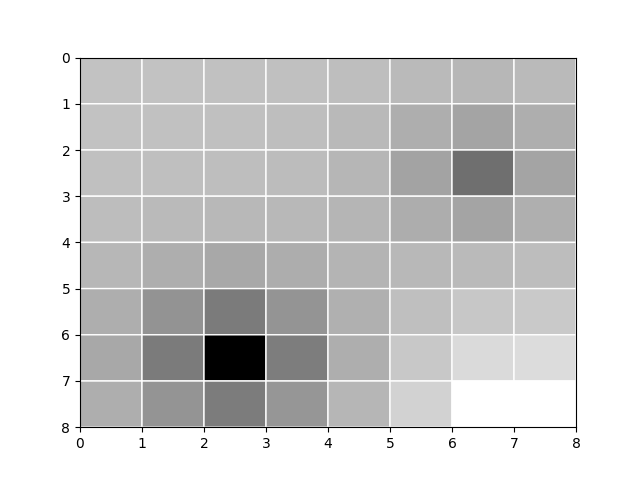
\includegraphics[width=1.\linewidth]{0_9.png}
	   \label{fig:grid_world2a}
	\end{minipage}\hfill
}
%\subfigure[]{
%	\begin{minipage}[c][0.85\width]{
%	   0.2\textwidth}
%	   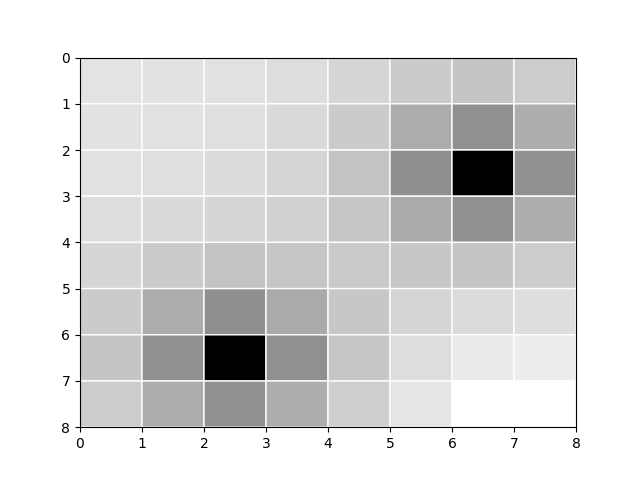
\includegraphics[width=1.2\linewidth]{0_8.png}
%	   \label{fig:grid_world2b}
%	\end{minipage}\hfill
%}
%\subfigure[]{
%	\begin{minipage}[c][0.85\width]{
%	   0.2\textwidth}
%	   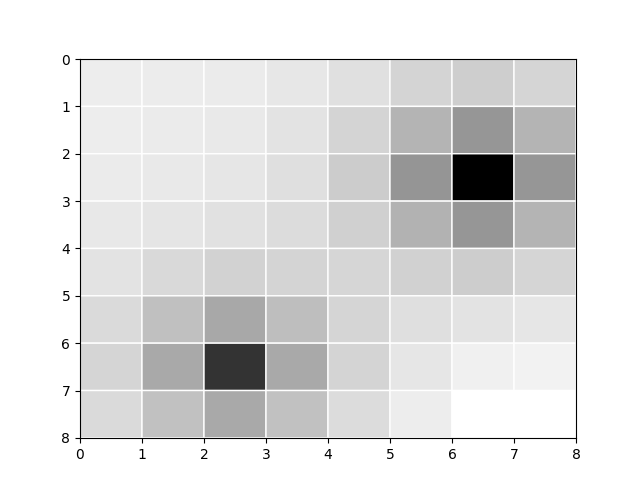
\includegraphics[width=1.2\linewidth]{0_6.png}
%	   \label{fig:grid_world2c}
%	\end{minipage}\hfill
%}
\subfigure[]{
	\begin{minipage}[c][0.8\width]{
	   0.3\textwidth}
	   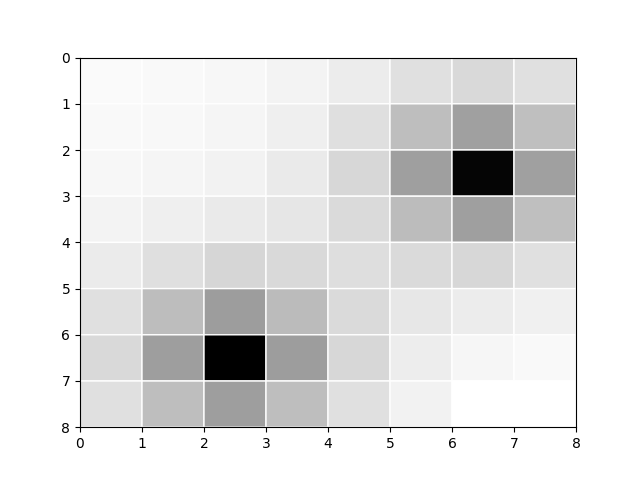
\includegraphics[width=1.\linewidth]{0_4.png}
	   \label{fig:grid_world2d}
	\end{minipage}\hfill
}
%\subfigure[]{
%	\begin{minipage}[c][0.85\width]{
%	   0.2\textwidth}
%	   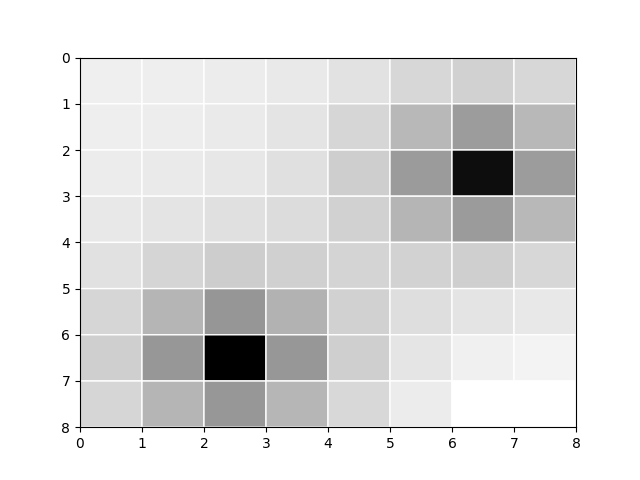
\includegraphics[width=1.2\linewidth]{0_2.png}
%	   \label{fig:grid_world2e}
%	\end{minipage}\hfill
%}
\subfigure[]{
	\begin{minipage}[c][0.8\width]{
	   0.3\textwidth}
	   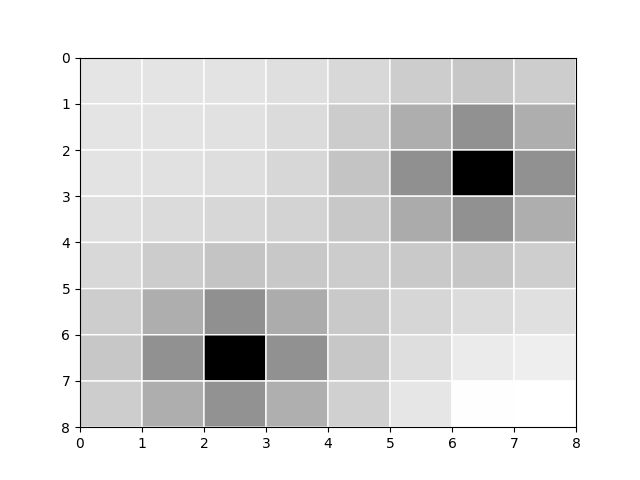
\includegraphics[width=1.\linewidth]{0_1.png}
	   \label{fig:grid_world2f}
	\end{minipage}\hspace{0.012\linewidth}
}
\caption[Reward mappings of gridworld for different safety threshold]
{(a)$p^* = 90\%$. The learnt policy has a probability of $12.5\%$ with respect to the given PCTL property. The reward function assigns lower rewards to the unsafe states than the states nearby. (b) $p^* = 40\%$. The learnt policy has a probability of $11.0\%$ with respect to the given PCTL property. The reward function assigns even lower rewards to the unsafe states, indicated by the greater contrast between unsafe states and other states. (c)$p^* = 10\%$. The learnt policy has a probability of $4\%$ with respect to the given PCTL property. The reward function assigns such low rewards to the unsafe states that the states nearby are also assigned with low rewards (because of the radial basis feature functions).}
\label{fig:grid_world2}
%\vspace{-4mm}
\end{figure}
%\vspace{-6mm}
\begin{table}[htb]
\begin{center}
\caption{Average runtime per iteration in seconds.}
\begin{tabular}{|c|r|r|r|r|r|}
\hline
Size & Num. of States & Compute $\pi$ & Compute $\mu$ & MC & Cex\\
\hline
$8 \times 8$ & 64 & 0.02 & 0.02 & 1.39 & 0.014\\
$16 \times 16$ & 256 & 0.05 & 0.05 & 1.43  & 0.014\\
$32 \times 32$ & 1024 & 0.07 & 0.08 & 3.12 & 0.035\\
$64 \times 64$ & 4096 & 6.52 & 25.88 &  22.877  & 1.59\\
\hline
\end{tabular}
\label{tab:grid-world}
\end{center}
\end{table}
%\vspace{-10mm}
We also evaluated the scalability of our implementation using the grid-world example. The first and second columns indicate the size of the grid world and the resulting state space. The third column shows the average runtime that policy iteration takes to compute an optimal policy $\pi$ for a known reward function. The forth column indicates the average runtime that policy iteration takes to compute the expected features $\mu$ for a known policy. The fifth column indicates the average runtime of verifying the PCTL formula using PRISM. The last column indicates the average runtime that generating a counterexample using COMICS.  


\section{Cart-Pole from OpenAI Gym}
%%\vspace{-8mm}
\begin{figure}[hbt]
  \centering
   	\subfigure[]{
	\begin{minipage}[c][0.35\textwidth]{
	   0.45\textwidth}
	   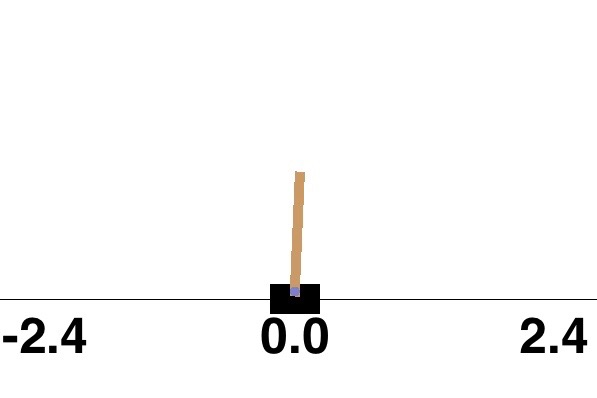
\includegraphics[width=\linewidth]{cartpole-v0.jpg}
	   \label{fig:cartpole-v0}
	\end{minipage}\hfill
}
\subfigure[]{
	\begin{minipage}[c][0.35\textwidth]{
	   0.45\textwidth}
	   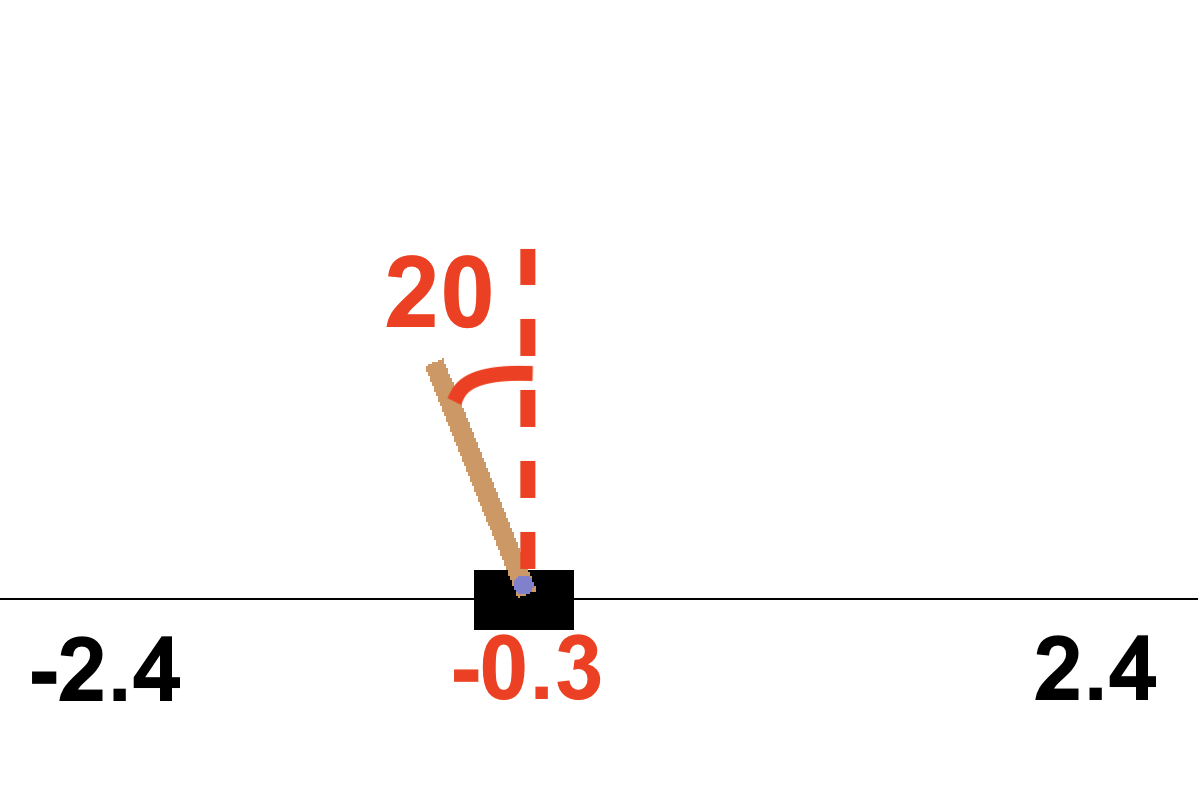
\includegraphics[width=\linewidth]{cartpole-v2.jpg}
	   \label{fig:cartpole-v1}
	\end{minipage}\hfill
}
\subfigure[]{
	\begin{minipage}[c][0.35\textwidth]{
	   0.45\textwidth}
	   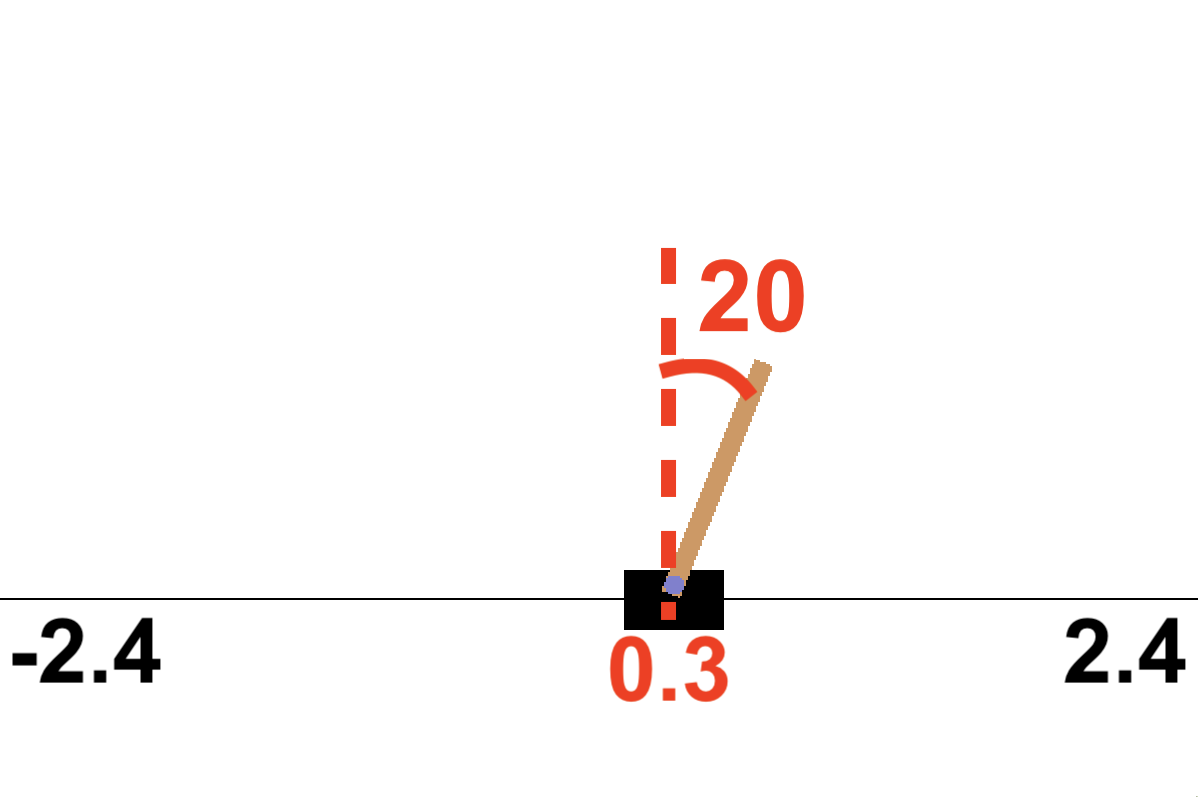
\includegraphics[width=\linewidth]{cartpole-v3.jpg}
	   \label{fig:cartpole-v2}
	\end{minipage}\hfill
}
%\vspace{-3mm} 
  \caption[The cartpole environment]{(a) The cartpole environment. (b) The cart is at -0.3 and pole angle is {-20}$^\circ$. (c) The cart is at 0.3 and pole angle is {20}$^\circ$.}    
\label{fig:cartpole}
%\vspace{-3mm}
\end{figure}
In grid world, it is hard to evaluate the performance that the agent may need to sacrifice for safety. Hence we implement the algorithm in OpenAI gym environments where performance can be quantified. In the cart-pole environment as shown in Fig.~\ref{fig:cartpole-v0}, the goal is to keep the pole on a cart from falling over as long as possible by moving the cart either to the left or to the right in each time step. The maximum step length is $t=200$. The position, velocity and angle of the cart and the pole are continuous values and observable, but the actual dynamics of the system are unknown.

We discretize the continuous observation space and formulate the environment as an MDP with 400 states and 2 actions. Through exploring the environment, the transition function is determined by the samples of experienced transitions. The feature vector in each state contains $30$ radial basis functions which depend on the squared Euclidean distances between current states and other $30$ states which are uniformly distributed in the state space. In addition, a maneuver is deemed {\it unsafe} if the pole angle is larger than 20$^\circ$ while the cart's horizontal position is more than $\pm 0.3$ as shown in Fig.~\ref{fig:cartpole-v1} and \ref{fig:cartpole-v2}. We formalize the safety requirement in PCTL as (\ref{eq:spec1}).
%\vspace{-2mm}
\begin{equation}
\begin{split}
\Phi ::= P_{\leq p^*}[true\ \until^{\leq t}\ &(angle\leq -20^\circ\wedge position\leq-0.3)\\
&\vee(angle\geq 20^\circ\wedge position\geq 0.3)]
\end{split}
\label{eq:spec1}
\end{equation}
%\vspace{-12mm}

\begin{table}[htb]
\begin{center}
\caption{In the cart-pole environment, {\it higher} average steps mean better performance. The safest policy is synthesized using PRISM-games.}
\begin{tabular}{|r|r|r|r|r|}
\hline
  &\small{\ \ MC Result} &\small{\ \ Avg. Steps}  &\small{\ \ Unsafe Rate} &\small{\ \ Num. of Iters}\\
\hline
AL &49.1\%& 165 &  19\% & 2\\
\hline
Safest Policy  & 0.0\% & 8 & 0.0\% & N.A.\\
\hline
$p^*=30\%$ & 17.2\%  & 121 & 13.0\% & 9\\
\hline
$p^*=25\%$ & 9.3\%  & 136 & 17.0\% & 13\\
\hline
$p^*=20\%$ & 17.2\% & 122 & 10.8\% & 8\\
\hline
$p^*=15\%$ & 7.3\% & 138 & 15.4\% & 21\\
\hline
$p^*=10\%$ & 7.2\% & 136 & 13.7\% & 21\\
\hline
$p^*=5\%$ & 0.04\% & 83 & 0.5\% & 50\\
\hline
\end{tabular}
\label{tab:cartpole1}
\end{center}
\end{table}
%\vspace{-10mm}

We consider only demonstrations for which the pole is held upright without violating any of the safety conditions for all 200 steps. The safest policy synthesized by PRISM-games is used as the initial safe policy. 
 We also compare the different policies learned by CEGAL for different safety threshold $p^*$s. 
In Table~\ref{tab:cartpole1}, the policies are compared in terms of model checking results (`MC Result') on the PCTL property in (\ref{eq:spec1}) using the constructed MDP, the average steps (`Avg. Steps') that a policy (executed in the OpenAI environment) can hold across $5000$ rounds (the higher the better), and averaged percentage times (`Unsafe Rate') that a policy (executed in the OpenAI environment) violates the $unsafe$ conditions across $5000$ rounds. The last column in the table shows the averaged number of iterations for these algorithms to converge (with $50$ as the maximum number of iterations). 
The policy in the first row is the result of using AL alone. 
Observe that from $p^* = 30\%$ to $10\%$, the performance of the learnt policy is similar. However, when the safety threshold becomes very low, e.g., $p^*=5\%$, the performance of the learnt policy drops significantly. 
Observe also that the safest policy has the lowest performance amongst all. 
It corresponds to simply letting the pole fall and thus does not risk moving the cart out of the range [-0.3, 0.3]. 
 We note that the discrepancy between the `MC result' and the `unsafe rate' is due to the MDP abstraction of the actual game environment. The safety guarantee of the algorithm is based on the former and the latter is used for validation purposes. The discordances between model checking results and unsafe rates are due to the inaccurate transition function. Despite the inconsistency, the policies learnt via CEGAL still show lower frequency of reaching unsafe states than that via AL.

\section{Mountain-Car from OpenAI Gym}
%\vspace{-5mm} 
\begin{figure}[h]
\centering
\subfigure[]{
	\hspace{0.1\linewidth}\begin{minipage}[c][0.35\textwidth]{
	   0.45\textwidth}
	   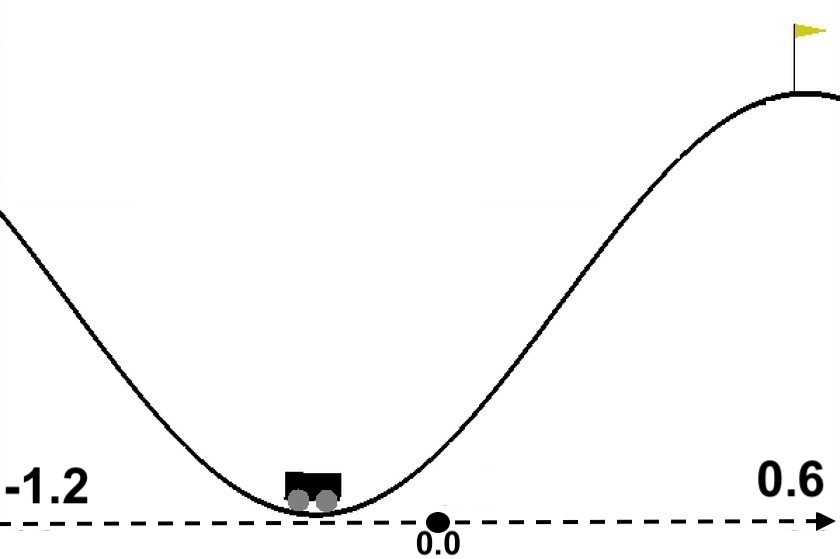
\includegraphics[width=1.2\linewidth]{mountaincar-v0.jpg}
	   \label{fig:mountaincar-v0}
	\end{minipage}\hspace{0.2\linewidth}
}
\subfigure[]{
	\begin{minipage}[c][0.35\textwidth]{
	   0.45\textwidth}
	   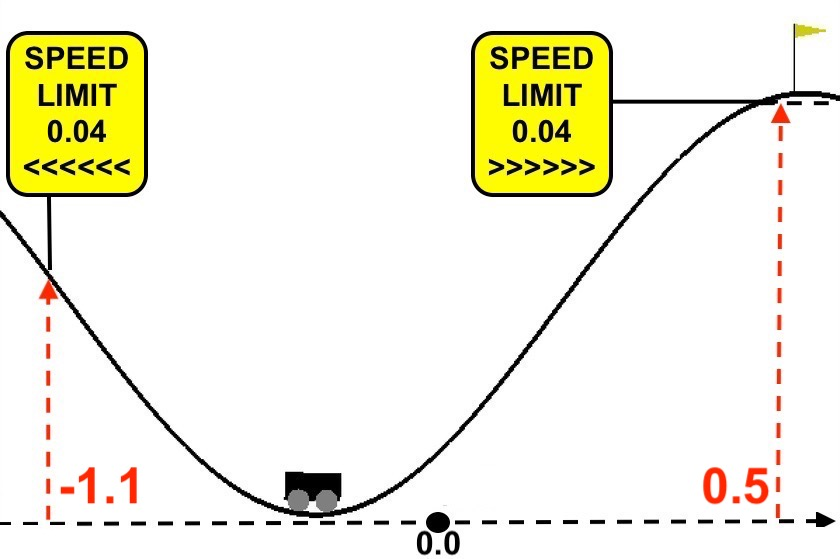
\includegraphics[width=1.2\linewidth]{mountaincar-v2.jpg}
	   \label{fig:mountaincar-v1}
	\end{minipage}\hspace{0.1\linewidth}
}
%\vspace{-3mm} 
\caption[The mountaincar environment]{(a) The original mountain-car environment. (b) The mountain-car environment with traffic rules: when the distance from the car to the left edge or the right edge is shorter than $0.1$, the speed of the car should be lower than $0.04$.}  
\label{fig:mountaincar}
\end{figure}

Our third experiment uses the mountain-car environment from OpenAI Gym. As shown in Fig. {\ref{fig:mountaincar-v0}}, a car starts from the bottom of the valley and tries to reach the mountaintop on the right as quickly as possible. In each time step the car can perform one of the three actions, accelerating to the left, coasting, and accelerating to the right. The agent fails if the step length reaches the maximum ($t=66$). The velocity and position of the car are continuous values and observable while the exact dynamics are unknown.

We discretize the continuous observation space and formulate the environment as an MDP with 320 states and 3 actions. Through exploring the environment, the transition function is determined by the samples of experienced transitions. The feature vector for each state contains 2 exponential functions and 18 radial basis functions which respectively depend on the squared Euclidean distances between the current state and other 18 states which are uniformly distributed in the state space. In this game setting, the car cannot reach the right mountaintop by simply accelerating to the right. It has to accumulate momentum first by moving back and forth in the valley. The safety rules we enforce are shown in Fig.~{\ref{fig:mountaincar-v1}. They correspond to speed limits when the car is close to the left mountaintop or to the right mountaintop (in case it is a cliff on the other side of the mountaintop). Similar to the previous experiments, we consider only expert demonstrations that successfully reach the right mountaintop without violating any of the safety conditions. 
The average step length of demonstrations is $40$. 
 We formalize the safety requirement in PCTL as (\ref{eq:spec2}). 

%\vspace{-5mm}
\begin{equation}
\begin{split}
\Phi ::= P_{\leq p^*}[true\ \until^{\leq t}\ &(speed\leq -0.04\wedge position\leq-1.1)\\
&\vee(speed\geq 0.04\wedge position\geq0.5)]
\end{split}
\label{eq:spec2}
\end{equation}
%\vspace{-2mm} 
\begin{table}[hbt]
\caption{In the mountain-car environment, {\it lower} average steps mean better performance. The safest policy is synthesized via PRISM-games.}
\begin{tabular}{|r|r|r|r|r|}
\hline 
\small{}  &\small{\ \ MC Result} &\small{\ \ Avg. Steps}  &\small{\ \ Unsafe Rate}&\small{\ \ Num. of Iters} \\ 
\hline \small
Policy Learnt via AL & 69.2\%& 54 & 100\% & 50\\
\hline
Safest Policy &  0.0\% &  $Fail$ & 0\% & 0\\
\hline
$p^*=60\%$&43.4\% & 57 & 33.2\% & 9\\
\hline
$p^*=50\%$ &46.9\%& 55 & 29.4\% & 23\\
\hline
$p^*=40\%$ &29.3\% & 61 & 0.6\% & 25\\
\hline
$p^*=30\%$ &18.9\% & 64 & 0.0\% & 17\\
\hline
$p^*=20\%$ &12.0\% & 66 & 3.5\% & 39\\
\hline
$p^*=10\%$ &7.6\% & $Fail$ & 0\%  & 40\\
\hline
\end{tabular}
\label{tab:mountaincar0}
%\vspace{-8mm}
\end{table}

 We compare the different policies using the same set of categories as in the cart-pole example. The numbers are averaged over 5000 rounds. The last column in the table shows the averaged number of iterations for these algorithms to converge (with $50$ as the maximum number of iterations).
As shown in the first row, the policy learnt via AL has the highest probability of going over the speed limits. We observe that this policy makes the car speed up all the way to the left mountaintop to maximize its potential energy. The safest policy corresponds to simply staying in the bottom of the valley. 
The policies learnt via CEGAL for the safety threshold $p^*$ ranges from $60\%$ to $50\%$ not only have lower probability of violating speed limits but also maintain comparable performance. However, when the safety threshold $p^*$ further decreases, the agent becomes more conservative and it takes more time for the car to finish the task. The discordances between model checking results and unsafe rates are due to the inaccurate transition function. Despite the inconsistency, the policies learnt via CEGAL still show obvious restraint in reaching unsafe states than that via AL.

\section{Discussion}
In the three experiments, we evaluate our algorithm in different aspects. From the gridworld experiment, we observe how safety specification influences the implicit search for reward function in our algorithm. When the safety threshold decreases, lower rewards will be assigned to the unsafe states so that the optimal policy with respect to the reward function will avoid reaching those states. From cart-pole and mountain-car experiments, we observe how our algorithm guarantees the safety of the final output policy while retaining the performance of the learnt policy in the mean time. In both experiments, by learning from human demonstrations and the counterexamples for violating the safety specification, the agent not only knows how to finish the tasks but also exhibits the awareness of safety.








\cleardoublepage

% -------------------------------------
% CHAPTER 3: CONCLUSION
% -------------------------------------
\chapter{Conclusions}
\label{chapter:Conclusions}
\thispagestyle{myheadings}

% set this to the location of the figures for this chapter. it may
% also want to be ../Figures/2_Body/ or something. make sure that
% it has a trailing directory separator (i.e., '/')!
\graphicspath{{3_Conclusion/Figures/}}

\section{Summary of the thesis}
In this thesis, a counterexample-guided approach is proposed for combining probabilistic model checking with apprenticeship learning to ensure safety of the learning outcome. By giving a safety specification and adding a verification oracle to the original apprenticeship learning algorithm, it is guaranteed that only a policy that satisfies the safety specification will be output. Furthermore, when a learnt policy is verified to violate the safety specification, a counterexample, which is a proof of the violation, will be extracted from the policy without risking deploying the unsafe policy in the field. Regarding counterexample as a negative example, the approach in this thesis makes novel use of the counterexamples to steer the policy search process by formulating the problem as a multi-objective optimization problem. By using an adaptive weight approach, the multi-objective optimization problem is solved iteratively and the multi-objective weight parameter is updated according to the learnt policy in each iteration. The algorithm is guaranteed to converge when the multi-objective weight parameter converges to a certain value. The experiment results indicate that the proposed approach can guarantee safety and retain performance for a set of benchmarks including examples drawn from OpenAI Gym.

However, the approach still has shortages in theories. One is lack of guarantee in finding a safe policy that performs as well as expert policy. Although it is natural that being safe can sometimes conflicts with high performance, I still need to find a boundary to leverage between different objects. For instance, in the multi-objective optimization problem, I used adaptive weighted sum approach. However, I didn't find the Pareto frontier for different $k$. Although I use constraints to ensure the dominance of the optimal $\pi$, $\hat{\pi}$ and $cex$ in individual iteration, more candidate policies and counterexamples will be found as the iteration continues. Thus, the dominance in one iteration may not hold in the future iteration. Another one shortage is the gap between the margin of policy features and margin of the true policy performance. In OpenAI gym environments, where performance can be quantified, a learnt policy that is {$\epsilon$-close} to the expert policy doesn't necessarily have performance comparable with expert policy. Whereas, this requires feature engineering, which is out of scope of this thesis. The last shortage s in the convergence of algorithm. By now, the convergence is fully based on the multi-objective parameter, which makes no guarantee in global optimum of the solved policy.

\section{Future Work}
In the future, firstly I'll try to deploy the algorithm and framework in realistic robotic control problems that have larger scale and are more complex than the OpenAI gym environments. Other than application, I would like to cover the theoretical shortages. For instance, I'll try to use gradient based method, rather than maximum margin principle, to solve apprenticeship learning problem and incorporate counterexample. Meanwhile, I would also like to explore other imitation or apprenticeship learning algorithms and extend our techniques to those settings. Last but not least, I would try different methods in policy verification and counterexample generation for substitutes to improve the scalability of the framework.


\cleardoublepage

%==========================================================================%
% Bibliography
\newpage
\singlespace
\bibliographystyle{apalike}

% each subdirectory can have its own BiBTeX file
\bibliography{thesis}
\cleardoublepage

%==========================================================================%
% Curriculum Vitae
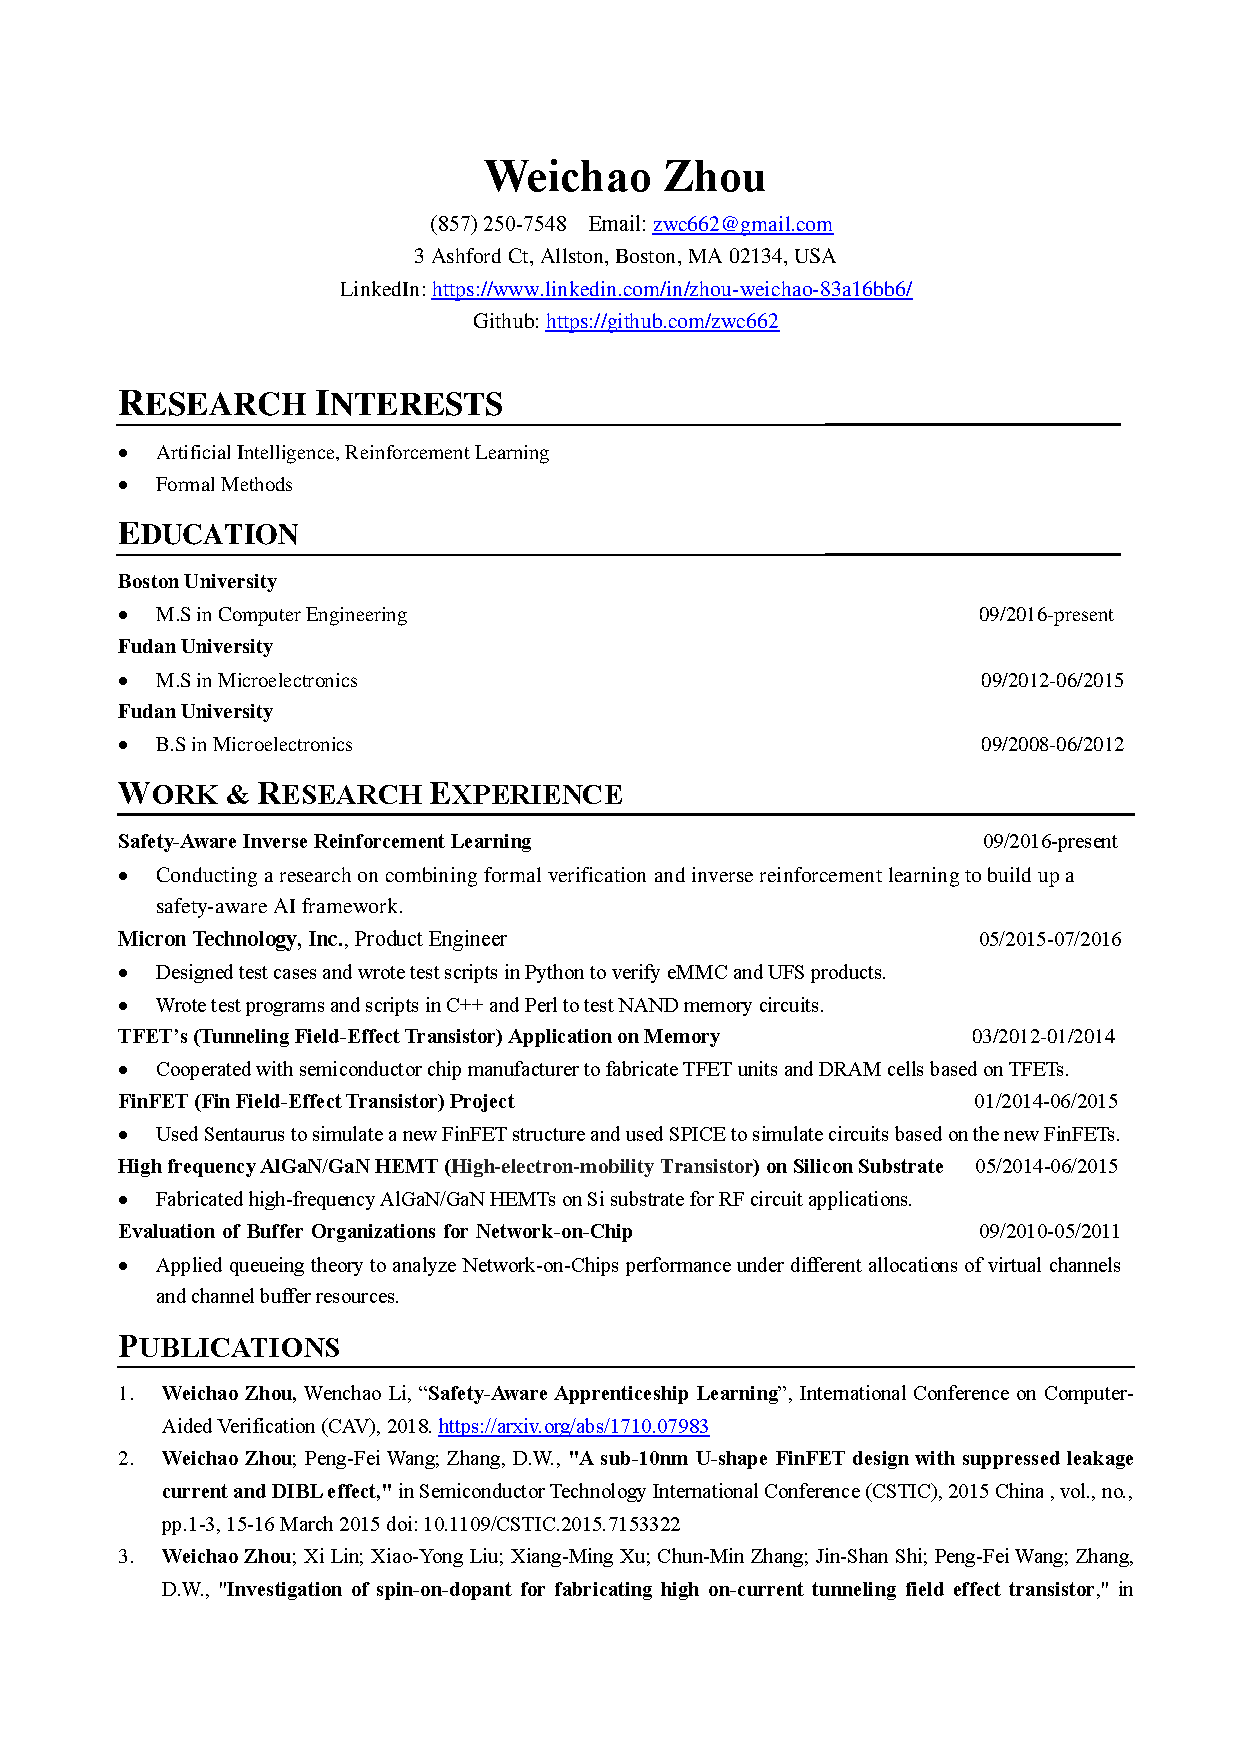
\includepdf{0_Prelim/cv} 

%==========================================================================%
\end{document}
